\documentclass[]{Book}
% The BYUPhys class is for producing theses and dissertations
% in the BYU Department of Physics and Astronomy.  You can supply
% the following optional arguments in the square brackets to
% specify the thesis type:
%
%   senior  : Produces the senior thesis preliminary pages (default)
%   honors  : Produces the honors thesis preliminary pages
%   masters : Produces the masters thesis preliminary pages
%   phd     : Produces the PhD dissertation preliminary pages
%
% The default format is appropriate for printing, with blank pages
% inserted after the preliminary pages in twoside mode so you can
% send it directly to a two-sided printer. However, for ETD
% submission the blank pages need to be removed from the final output.
% The following option does this for you:
%
%   etd     : Produces a copy with no blank pages in the preliminary section.
%             Remove this option to produce a version with blank pages inserted
%             for easy double sided printing.
%
% The rest of the class options are the same as the regular book class.
% A few to remember:
%
%   oneside : Produces single sided print layout (recommended for theses less than 50 pages)
%   twoside : Produces single sided print layout (the default if you remove oneside)
%
% The BYUPhys class provides the following macros:
%
%   \makepreliminarypages : Makes the preliminary pages
%   \clearemptydoublepage : same as \cleardoublepage but doesn't put page numbers
%                           on blank intervening pages
%   \singlespace          : switch to single spaced lines
%   \doublespace          : switch to double spaced lines
%
% --------------------------- Load Packages ---------------------------------

% The graphicx package allows the inclusion of figures.  Plain LaTeX and
% pdfLaTeX handle graphics differently. The following code checks which one
% you are compiling with, and switches the graphicx package options accordingly.
\usepackage{ifpdf}
\ifpdf
  \usepackage[pdftex]{graphicx}
\else
  \usepackage[dvips]{graphicx}
\fi

% The fancyhdr package allows you to easily customize the page header.
% The settings below produce a nice, well separated header.
\usepackage{fancyhdr}
  \fancyhead{}
  \fancyhead[LO]{\slshape \rightmark}
  \fancyhead[RO,LE]{\textbf{\thepage}}
  \fancyhead[RE]{\slshape \leftmark}
  \fancyfoot{}
  \pagestyle{fancy}
  \renewcommand{\chaptermark}[1]{\markboth{\chaptername \ \thechapter \ \ #1}{}}
  \renewcommand{\sectionmark}[1]{\markright{\thesection \ \ #1}}

% The caption package allows us to change the formatting of figure captions.
% The commands here change to the suggested caption format: single spaced and a bold tag
\usepackage[margin=0.3in,labelfont=bf,labelsep=none]{caption}
 \DeclareCaptionFormat{suggested}{\singlespace#1#2 #3\par\doublespace}
 \captionsetup{format=suggested}

% The cite package cleans up the way citations are handled.  For example, it
% changes the citation [1,2,3,6,7,8,9,10,11] into [1-3,6-11].  If your advisor
% wants superscript citations, use the overcite package instead of the cite package.
\usepackage[noadjust]{cite}

% The makeidx package makes your index for you.  To make an index entry,
% go to the place in the book that should be referenced and type
%  \index{key}
% An index entry labeled "key" (or whatever you type) will then
% be included and point to the correct page.
\usepackage{makeidx}
\makeindex

% The url package allows for the nice typesetting of URLs.  Since URLs are often
% long with no spaces, they mess up line wrapping.  The command \url{http://www.physics.byu.edu}
% allows LaTeX to break the url across lines at appropriate places: e.g. http://www.
% physics.byu.edu.  This is helpful if you reference web pages.
\usepackage{url}
\urlstyle{rm}

% If you have a lot of equations, you might be interested in the amstex package.
% It defines a number of environments and macros that are helpful for mathematics.
% We don't do much math in this example, so we haven't used amstex here.
\usepackage{amsmath}

% If you need chemistry symbols you can use \usepackage{mhchem} to make them. They are made in the following way \ce{ H2O }
\usepackage{mhchem}


% The hyperref package provides automatic linking and bookmarking for the table
% of contents, index, equation references, and figure references.  It must be
% included for the BYU Physics class to make a properly functioning electronic
% thesis.  It should be the last package loaded if possible.
%
% To include a link in your pdf use \href{URL}{Text to be displayed}.  If your
% display text is the URL, you probably should use the \url{} command discussed
% above.
%
% To add a bookmark in the pdf you can use \pdfbookmark.  You can look up its usage
% in the hyperref package documentation
\usepackage[bookmarksnumbered,pdfpagelabels=true,plainpages=false,colorlinks=true,
            linkcolor=black,citecolor=black,urlcolor=blue]{hyperref}

% ------------------------- Fill in these fields for the preliminary pages ----------------------------
%
% try to fix the tci macro problem
% Macros for Scientific Word and Scientific WorkPlace 5.5 documents saved with the LaTeX filter.
% Copyright (C) 2005 Mackichan Software, Inc.

\typeout{TCILATEX Macros for Scientific Word and Scientific WorkPlace 5.5 <06 Oct 2005>.}
\typeout{NOTICE:  This macro file is NOT proprietary and may be 
freely copied and distributed.}
%
\makeatletter

%%%%%%%%%%%%%%%%%%%%%
% pdfTeX related.
\ifx\pdfoutput\relax\let\pdfoutput=\undefined\fi
\newcount\msipdfoutput
\ifx\pdfoutput\undefined
\else
 \ifcase\pdfoutput
 \else 
    \msipdfoutput=1
    \ifx\paperwidth\undefined
    \else
      \ifdim\paperheight=0pt\relax
      \else
        \pdfpageheight\paperheight
      \fi
      \ifdim\paperwidth=0pt\relax
      \else
        \pdfpagewidth\paperwidth
      \fi
    \fi
  \fi  
\fi

%%%%%%%%%%%%%%%%%%%%%
% FMTeXButton
% This is used for putting TeXButtons in the 
% frontmatter of a document. Add a line like
% \QTagDef{FMTeXButton}{101}{} to the filter 
% section of the cst being used. Also add a
% new section containing:
%     [f_101]
%     ALIAS=FMTexButton
%     TAG_TYPE=FIELD
%     TAG_LEADIN=TeX Button:
%
% It also works to put \defs in the preamble after 
% the \input tcilatex
\def\FMTeXButton#1{#1}
%
%%%%%%%%%%%%%%%%%%%%%%
% macros for time
\newcount\@hour\newcount\@minute\chardef\@x10\chardef\@xv60
\def\tcitime{
\def\@time{%
  \@minute\time\@hour\@minute\divide\@hour\@xv
  \ifnum\@hour<\@x 0\fi\the\@hour:%
  \multiply\@hour\@xv\advance\@minute-\@hour
  \ifnum\@minute<\@x 0\fi\the\@minute
  }}%

%%%%%%%%%%%%%%%%%%%%%%
% macro for hyperref and msihyperref
%\@ifundefined{hyperref}{\def\hyperref#1#2#3#4{#2\ref{#4}#3}}{}

\def\x@hyperref#1#2#3{%
   % Turn off various catcodes before reading parameter 4
   \catcode`\~ = 12
   \catcode`\$ = 12
   \catcode`\_ = 12
   \catcode`\# = 12
   \catcode`\& = 12
   \catcode`\% = 12
   \y@hyperref{#1}{#2}{#3}%
}

\def\y@hyperref#1#2#3#4{%
   #2\ref{#4}#3
   \catcode`\~ = 13
   \catcode`\$ = 3
   \catcode`\_ = 8
   \catcode`\# = 6
   \catcode`\& = 4
   \catcode`\% = 14
}

\@ifundefined{hyperref}{\let\hyperref\x@hyperref}{}
\@ifundefined{msihyperref}{\let\msihyperref\x@hyperref}{}




% macro for external program call
\@ifundefined{qExtProgCall}{\def\qExtProgCall#1#2#3#4#5#6{\relax}}{}
%%%%%%%%%%%%%%%%%%%%%%
%
% macros for graphics
%
\def\FILENAME#1{#1}%
%
\def\QCTOpt[#1]#2{%
  \def\QCTOptB{#1}
  \def\QCTOptA{#2}
}
\def\QCTNOpt#1{%
  \def\QCTOptA{#1}
  \let\QCTOptB\empty
}
\def\Qct{%
  \@ifnextchar[{%
    \QCTOpt}{\QCTNOpt}
}
\def\QCBOpt[#1]#2{%
  \def\QCBOptB{#1}%
  \def\QCBOptA{#2}%
}
\def\QCBNOpt#1{%
  \def\QCBOptA{#1}%
  \let\QCBOptB\empty
}
\def\Qcb{%
  \@ifnextchar[{%
    \QCBOpt}{\QCBNOpt}%
}
\def\PrepCapArgs{%
  \ifx\QCBOptA\empty
    \ifx\QCTOptA\empty
      {}%
    \else
      \ifx\QCTOptB\empty
        {\QCTOptA}%
      \else
        [\QCTOptB]{\QCTOptA}%
      \fi
    \fi
  \else
    \ifx\QCBOptA\empty
      {}%
    \else
      \ifx\QCBOptB\empty
        {\QCBOptA}%
      \else
        [\QCBOptB]{\QCBOptA}%
      \fi
    \fi
  \fi
}
\newcount\GRAPHICSTYPE
%\GRAPHICSTYPE 0 is for TurboTeX
%\GRAPHICSTYPE 1 is for DVIWindo (PostScript)
%%%(removed)%\GRAPHICSTYPE 2 is for psfig (PostScript)
\GRAPHICSTYPE=\z@
\def\GRAPHICSPS#1{%
 \ifcase\GRAPHICSTYPE%\GRAPHICSTYPE=0
   \special{ps: #1}%
 \or%\GRAPHICSTYPE=1
   \special{language "PS", include "#1"}%
%%%\or%\GRAPHICSTYPE=2
%%%  #1%
 \fi
}%
%
\def\GRAPHICSHP#1{\special{include #1}}%
%
% \graffile{ body }                                  %#1
%          { contentswidth (scalar)  }               %#2
%          { contentsheight (scalar) }               %#3
%          { vertical shift when in-line (scalar) }  %#4

\def\graffile#1#2#3#4{%
%%% \ifnum\GRAPHICSTYPE=\tw@
%%%  %Following if using psfig
%%%  \@ifundefined{psfig}{\input psfig.tex}{}%
%%%  \psfig{file=#1, height=#3, width=#2}%
%%% \else
  %Following for all others
  % JCS - added BOXTHEFRAME, see below
    \bgroup
	   \@inlabelfalse
       \leavevmode
       \@ifundefined{bbl@deactivate}{\def~{\string~}}{\activesoff}%
        \raise -#4 \BOXTHEFRAME{%
           \hbox to #2{\raise #3\hbox to #2{\null #1\hfil}}}%
    \egroup
}%
%
% A box for drafts
\def\draftbox#1#2#3#4{%
 \leavevmode\raise -#4 \hbox{%
  \frame{\rlap{\protect\tiny #1}\hbox to #2%
   {\vrule height#3 width\z@ depth\z@\hfil}%
  }%
 }%
}%
%
\newcount\@msidraft
\@msidraft=\z@
\let\nographics=\@msidraft
\newif\ifwasdraft
\wasdraftfalse

%  \GRAPHIC{ body }                                  %#1
%          { draft name }                            %#2
%          { contentswidth (scalar)  }               %#3
%          { contentsheight (scalar) }               %#4
%          { vertical shift when in-line (scalar) }  %#5
\def\GRAPHIC#1#2#3#4#5{%
   \ifnum\@msidraft=\@ne\draftbox{#2}{#3}{#4}{#5}%
   \else\graffile{#1}{#3}{#4}{#5}%
   \fi
}
%
\def\addtoLaTeXparams#1{%
    \edef\LaTeXparams{\LaTeXparams #1}}%
%
% JCS -  added a switch BoxFrame that can 
% be set by including X in the frame params.
% If set a box is drawn around the frame.

\newif\ifBoxFrame \BoxFramefalse
\newif\ifOverFrame \OverFramefalse
\newif\ifUnderFrame \UnderFramefalse

\def\BOXTHEFRAME#1{%
   \hbox{%
      \ifBoxFrame
         \frame{#1}%
      \else
         {#1}%
      \fi
   }%
}


\def\doFRAMEparams#1{\BoxFramefalse\OverFramefalse\UnderFramefalse\readFRAMEparams#1\end}%
\def\readFRAMEparams#1{%
 \ifx#1\end%
  \let\next=\relax
  \else
  \ifx#1i\dispkind=\z@\fi
  \ifx#1d\dispkind=\@ne\fi
  \ifx#1f\dispkind=\tw@\fi
  \ifx#1t\addtoLaTeXparams{t}\fi
  \ifx#1b\addtoLaTeXparams{b}\fi
  \ifx#1p\addtoLaTeXparams{p}\fi
  \ifx#1h\addtoLaTeXparams{h}\fi
  \ifx#1X\BoxFrametrue\fi
  \ifx#1O\OverFrametrue\fi
  \ifx#1U\UnderFrametrue\fi
  \ifx#1w
    \ifnum\@msidraft=1\wasdrafttrue\else\wasdraftfalse\fi
    \@msidraft=\@ne
  \fi
  \let\next=\readFRAMEparams
  \fi
 \next
 }%
%
%Macro for In-line graphics object
%   \IFRAME{ contentswidth (scalar)  }               %#1
%          { contentsheight (scalar) }               %#2
%          { vertical shift when in-line (scalar) }  %#3
%          { draft name }                            %#4
%          { body }                                  %#5
%          { caption}                                %#6


\def\IFRAME#1#2#3#4#5#6{%
      \bgroup
      \let\QCTOptA\empty
      \let\QCTOptB\empty
      \let\QCBOptA\empty
      \let\QCBOptB\empty
      #6%
      \parindent=0pt
      \leftskip=0pt
      \rightskip=0pt
      \setbox0=\hbox{\QCBOptA}%
      \@tempdima=#1\relax
      \ifOverFrame
          % Do this later
          \typeout{This is not implemented yet}%
          \show\HELP
      \else
         \ifdim\wd0>\@tempdima
            \advance\@tempdima by \@tempdima
            \ifdim\wd0 >\@tempdima
               \setbox1 =\vbox{%
                  \unskip\hbox to \@tempdima{\hfill\GRAPHIC{#5}{#4}{#1}{#2}{#3}\hfill}%
                  \unskip\hbox to \@tempdima{\parbox[b]{\@tempdima}{\QCBOptA}}%
               }%
               \wd1=\@tempdima
            \else
               \textwidth=\wd0
               \setbox1 =\vbox{%
                 \noindent\hbox to \wd0{\hfill\GRAPHIC{#5}{#4}{#1}{#2}{#3}\hfill}\\%
                 \noindent\hbox{\QCBOptA}%
               }%
               \wd1=\wd0
            \fi
         \else
            \ifdim\wd0>0pt
              \hsize=\@tempdima
              \setbox1=\vbox{%
                \unskip\GRAPHIC{#5}{#4}{#1}{#2}{0pt}%
                \break
                \unskip\hbox to \@tempdima{\hfill \QCBOptA\hfill}%
              }%
              \wd1=\@tempdima
           \else
              \hsize=\@tempdima
              \setbox1=\vbox{%
                \unskip\GRAPHIC{#5}{#4}{#1}{#2}{0pt}%
              }%
              \wd1=\@tempdima
           \fi
         \fi
         \@tempdimb=\ht1
         %\advance\@tempdimb by \dp1
         \advance\@tempdimb by -#2
         \advance\@tempdimb by #3
         \leavevmode
         \raise -\@tempdimb \hbox{\box1}%
      \fi
      \egroup%
}%
%
%Macro for Display graphics object
%   \DFRAME{ contentswidth (scalar)  }               %#1
%          { contentsheight (scalar) }               %#2
%          { draft label }                           %#3
%          { name }                                  %#4
%          { caption}                                %#5
\def\DFRAME#1#2#3#4#5{%
  \vspace\topsep
  \hfil\break
  \bgroup
     \leftskip\@flushglue
	 \rightskip\@flushglue
	 \parindent\z@
	 \parfillskip\z@skip
     \let\QCTOptA\empty
     \let\QCTOptB\empty
     \let\QCBOptA\empty
     \let\QCBOptB\empty
	 \vbox\bgroup
        \ifOverFrame 
           #5\QCTOptA\par
        \fi
        \GRAPHIC{#4}{#3}{#1}{#2}{\z@}%
        \ifUnderFrame 
           \break#5\QCBOptA
        \fi
	 \egroup
  \egroup
  \vspace\topsep
  \break
}%
%
%Macro for Floating graphic object
%   \FFRAME{ framedata f|i tbph x F|T }              %#1
%          { contentswidth (scalar)  }               %#2
%          { contentsheight (scalar) }               %#3
%          { caption }                               %#4
%          { label }                                 %#5
%          { draft name }                            %#6
%          { body }                                  %#7
\def\FFRAME#1#2#3#4#5#6#7{%
 %If float.sty loaded and float option is 'h', change to 'H'  (gp) 1998/09/05
  \@ifundefined{floatstyle}
    {%floatstyle undefined (and float.sty not present), no change
     \begin{figure}[#1]%
    }
    {%floatstyle DEFINED
	 \ifx#1h%Only the h parameter, change to H
      \begin{figure}[H]%
	 \else
      \begin{figure}[#1]%
	 \fi
	}
  \let\QCTOptA\empty
  \let\QCTOptB\empty
  \let\QCBOptA\empty
  \let\QCBOptB\empty
  \ifOverFrame
    #4
    \ifx\QCTOptA\empty
    \else
      \ifx\QCTOptB\empty
        \caption{\QCTOptA}%
      \else
        \caption[\QCTOptB]{\QCTOptA}%
      \fi
    \fi
    \ifUnderFrame\else
      \label{#5}%
    \fi
  \else
    \UnderFrametrue%
  \fi
  \begin{center}\GRAPHIC{#7}{#6}{#2}{#3}{\z@}\end{center}%
  \ifUnderFrame
    #4
    \ifx\QCBOptA\empty
      \caption{}%
    \else
      \ifx\QCBOptB\empty
        \caption{\QCBOptA}%
      \else
        \caption[\QCBOptB]{\QCBOptA}%
      \fi
    \fi
    \label{#5}%
  \fi
  \end{figure}%
 }%
%
%
%    \FRAME{ framedata f|i tbph x F|T }              %#1
%          { contentswidth (scalar)  }               %#2
%          { contentsheight (scalar) }               %#3
%          { vertical shift when in-line (scalar) }  %#4
%          { caption }                               %#5
%          { label }                                 %#6
%          { name }                                  %#7
%          { body }                                  %#8
%
%    framedata is a string which can contain the following
%    characters: idftbphxFT
%    Their meaning is as follows:
%             i, d or f : in-line, display, or floating
%             t,b,p,h   : LaTeX floating placement options
%             x         : fit contents box to contents
%             F or T    : Figure or Table. 
%                         Later this can expand
%                         to a more general float class.
%
%
\newcount\dispkind%

\def\makeactives{
  \catcode`\"=\active
  \catcode`\;=\active
  \catcode`\:=\active
  \catcode`\'=\active
  \catcode`\~=\active
}
\bgroup
   \makeactives
   \gdef\activesoff{%
      \def"{\string"}%
      \def;{\string;}%
      \def:{\string:}%
      \def'{\string'}%
      \def~{\string~}%
      %\bbl@deactivate{"}%
      %\bbl@deactivate{;}%
      %\bbl@deactivate{:}%
      %\bbl@deactivate{'}%
    }
\egroup

\def\FRAME#1#2#3#4#5#6#7#8{%
 \bgroup
 \ifnum\@msidraft=\@ne
   \wasdrafttrue
 \else
   \wasdraftfalse%
 \fi
 \def\LaTeXparams{}%
 \dispkind=\z@
 \def\LaTeXparams{}%
 \doFRAMEparams{#1}%
 \ifnum\dispkind=\z@\IFRAME{#2}{#3}{#4}{#7}{#8}{#5}\else
  \ifnum\dispkind=\@ne\DFRAME{#2}{#3}{#7}{#8}{#5}\else
   \ifnum\dispkind=\tw@
    \edef\@tempa{\noexpand\FFRAME{\LaTeXparams}}%
    \@tempa{#2}{#3}{#5}{#6}{#7}{#8}%
    \fi
   \fi
  \fi
  \ifwasdraft\@msidraft=1\else\@msidraft=0\fi{}%
  \egroup
 }%
%
% This macro added to let SW gobble a parameter that
% should not be passed on and expanded. 

\def\TEXUX#1{"texux"}

%
% Macros for text attributes:
%
\def\BF#1{{\bf {#1}}}%
\def\NEG#1{\leavevmode\hbox{\rlap{\thinspace/}{$#1$}}}%
%
%%%%%%%%%%%%%%%%%%%%%%%%%%%%%%%%%%%%%%%%%%%%%%%%%%%%%%%%%%%%%%%%%%%%%%%%
%
%
% macros for user - defined functions
\def\limfunc#1{\mathop{\rm #1}}%
\def\func#1{\mathop{\rm #1}\nolimits}%
% macro for unit names
\def\unit#1{\mathord{\thinspace\rm #1}}%

%
% miscellaneous 
\long\def\QQQ#1#2{%
     \long\expandafter\def\csname#1\endcsname{#2}}%
\@ifundefined{QTP}{\def\QTP#1{}}{}
\@ifundefined{QEXCLUDE}{\def\QEXCLUDE#1{}}{}
\@ifundefined{Qlb}{\def\Qlb#1{#1}}{}
\@ifundefined{Qlt}{\def\Qlt#1{#1}}{}
\def\QWE{}%
\long\def\QQA#1#2{}%
\def\QTR#1#2{{\csname#1\endcsname {#2}}}%
  %	Add aliases for the ulem package
  \let\QQQuline\uline
  \let\QQQsout\sout
  \let\QQQuuline\uuline
  \let\QQQuwave\uwave
  \let\QQQxout\xout
\long\def\TeXButton#1#2{#2}%
\long\def\QSubDoc#1#2{#2}%
\def\EXPAND#1[#2]#3{}%
\def\NOEXPAND#1[#2]#3{}%
\def\PROTECTED{}%
\def\LaTeXparent#1{}%
\def\ChildStyles#1{}%
\def\ChildDefaults#1{}%
\def\QTagDef#1#2#3{}%

% Constructs added with Scientific Notebook
\@ifundefined{correctchoice}{\def\correctchoice{\relax}}{}
\@ifundefined{HTML}{\def\HTML#1{\relax}}{}
\@ifundefined{TCIIcon}{\def\TCIIcon#1#2#3#4{\relax}}{}
\if@compatibility
  \typeout{Not defining UNICODE  U or CustomNote commands for LaTeX 2.09.}
\else
  \providecommand{\UNICODE}[2][]{\protect\rule{.1in}{.1in}}
  \providecommand{\U}[1]{\protect\rule{.1in}{.1in}}
  \providecommand{\CustomNote}[3][]{\marginpar{#3}}
\fi

\@ifundefined{lambdabar}{
      \def\lambdabar{\errmessage{You have used the lambdabar symbol. 
                      This is available for typesetting only in RevTeX styles.}}
   }{}

%
% Macros for style editor docs
\@ifundefined{StyleEditBeginDoc}{\def\StyleEditBeginDoc{\relax}}{}
%
% Macros for footnotes
\def\QQfnmark#1{\footnotemark}
\def\QQfntext#1#2{\addtocounter{footnote}{#1}\footnotetext{#2}}
%
% Macros for indexing.
%
\@ifundefined{TCIMAKEINDEX}{}{\makeindex}%
%
% Attempts to avoid problems with other styles
\@ifundefined{abstract}{%
 \def\abstract{%
  \if@twocolumn
   \section*{Abstract (Not appropriate in this style!)}%
   \else \small 
   \begin{center}{\bf Abstract\vspace{-.5em}\vspace{\z@}}\end{center}%
   \quotation 
   \fi
  }%
 }{%
 }%
\@ifundefined{endabstract}{\def\endabstract
  {\if@twocolumn\else\endquotation\fi}}{}%
\@ifundefined{maketitle}{\def\maketitle#1{}}{}%
\@ifundefined{affiliation}{\def\affiliation#1{}}{}%
\@ifundefined{proof}{\def\proof{\noindent{\bfseries Proof. }}}{}%
\@ifundefined{endproof}{\def\endproof{\mbox{\ \rule{.1in}{.1in}}}}{}%
\@ifundefined{newfield}{\def\newfield#1#2{}}{}%
\@ifundefined{chapter}{\def\chapter#1{\par(Chapter head:)#1\par }%
 \newcount\c@chapter}{}%
\@ifundefined{part}{\def\part#1{\par(Part head:)#1\par }}{}%
\@ifundefined{section}{\def\section#1{\par(Section head:)#1\par }}{}%
\@ifundefined{subsection}{\def\subsection#1%
 {\par(Subsection head:)#1\par }}{}%
\@ifundefined{subsubsection}{\def\subsubsection#1%
 {\par(Subsubsection head:)#1\par }}{}%
\@ifundefined{paragraph}{\def\paragraph#1%
 {\par(Subsubsubsection head:)#1\par }}{}%
\@ifundefined{subparagraph}{\def\subparagraph#1%
 {\par(Subsubsubsubsection head:)#1\par }}{}%
%%%%%%%%%%%%%%%%%%%%%%%%%%%%%%%%%%%%%%%%%%%%%%%%%%%%%%%%%%%%%%%%%%%%%%%%
% These symbols are not recognized by LaTeX
\@ifundefined{therefore}{\def\therefore{}}{}%
\@ifundefined{backepsilon}{\def\backepsilon{}}{}%
\@ifundefined{yen}{\def\yen{\hbox{\rm\rlap=Y}}}{}%
\@ifundefined{registered}{%
   \def\registered{\relax\ifmmode{}\r@gistered
                    \else$\m@th\r@gistered$\fi}%
 \def\r@gistered{^{\ooalign
  {\hfil\raise.07ex\hbox{$\scriptstyle\rm\text{R}$}\hfil\crcr
  \mathhexbox20D}}}}{}%
\@ifundefined{Eth}{\def\Eth{}}{}%
\@ifundefined{eth}{\def\eth{}}{}%
\@ifundefined{Thorn}{\def\Thorn{}}{}%
\@ifundefined{thorn}{\def\thorn{}}{}%
% A macro to allow any symbol that requires math to appear in text
\def\TEXTsymbol#1{\mbox{$#1$}}%
\@ifundefined{degree}{\def\degree{{}^{\circ}}}{}%
%
% macros for T3TeX files
\newdimen\theight
\@ifundefined{Column}{\def\Column{%
 \vadjust{\setbox\z@=\hbox{\scriptsize\quad\quad tcol}%
  \theight=\ht\z@\advance\theight by \dp\z@\advance\theight by \lineskip
  \kern -\theight \vbox to \theight{%
   \rightline{\rlap{\box\z@}}%
   \vss
   }%
  }%
 }}{}%
%
\@ifundefined{qed}{\def\qed{%
 \ifhmode\unskip\nobreak\fi\ifmmode\ifinner\else\hskip5\p@\fi\fi
 \hbox{\hskip5\p@\vrule width4\p@ height6\p@ depth1.5\p@\hskip\p@}%
 }}{}%
%
\@ifundefined{cents}{\def\cents{\hbox{\rm\rlap c/}}}{}%
\@ifundefined{tciLaplace}{\def\tciLaplace{\ensuremath{\mathcal{L}}}}{}%
\@ifundefined{tciFourier}{\def\tciFourier{\ensuremath{\mathcal{F}}}}{}%
\@ifundefined{textcurrency}{\def\textcurrency{\hbox{\rm\rlap xo}}}{}%
\@ifundefined{texteuro}{\def\texteuro{\hbox{\rm\rlap C=}}}{}%
\@ifundefined{euro}{\def\euro{\hbox{\rm\rlap C=}}}{}%
\@ifundefined{textfranc}{\def\textfranc{\hbox{\rm\rlap-F}}}{}%
\@ifundefined{textlira}{\def\textlira{\hbox{\rm\rlap L=}}}{}%
\@ifundefined{textpeseta}{\def\textpeseta{\hbox{\rm P\negthinspace s}}}{}%
%
\@ifundefined{miss}{\def\miss{\hbox{\vrule height2\p@ width 2\p@ depth\z@}}}{}%
%
\@ifundefined{vvert}{\def\vvert{\Vert}}{}%  %always translated to \left| or \right|
%
\@ifundefined{tcol}{\def\tcol#1{{\baselineskip=6\p@ \vcenter{#1}} \Column}}{}%
%
\@ifundefined{dB}{\def\dB{\hbox{{}}}}{}%        %dummy entry in column 
\@ifundefined{mB}{\def\mB#1{\hbox{$#1$}}}{}%   %column entry
\@ifundefined{nB}{\def\nB#1{\hbox{#1}}}{}%     %column entry (not math)
%
\@ifundefined{note}{\def\note{$^{\dag}}}{}%
%
\def\newfmtname{LaTeX2e}
% No longer load latexsym.  This is now handled by SWP, which uses amsfonts if necessary
%
\ifx\fmtname\newfmtname
  \DeclareOldFontCommand{\rm}{\normalfont\rmfamily}{\mathrm}
  \DeclareOldFontCommand{\sf}{\normalfont\sffamily}{\mathsf}
  \DeclareOldFontCommand{\tt}{\normalfont\ttfamily}{\mathtt}
  \DeclareOldFontCommand{\bf}{\normalfont\bfseries}{\mathbf}
  \DeclareOldFontCommand{\it}{\normalfont\itshape}{\mathit}
  \DeclareOldFontCommand{\sl}{\normalfont\slshape}{\@nomath\sl}
  \DeclareOldFontCommand{\sc}{\normalfont\scshape}{\@nomath\sc}
\fi

%
% Greek bold macros
% Redefine all of the math symbols 
% which might be bolded	 - there are 
% probably others to add to this list

\def\alpha{{\Greekmath 010B}}%
\def\beta{{\Greekmath 010C}}%
\def\gamma{{\Greekmath 010D}}%
\def\delta{{\Greekmath 010E}}%
\def\epsilon{{\Greekmath 010F}}%
\def\zeta{{\Greekmath 0110}}%
\def\eta{{\Greekmath 0111}}%
\def\theta{{\Greekmath 0112}}%
\def\iota{{\Greekmath 0113}}%
\def\kappa{{\Greekmath 0114}}%
\def\lambda{{\Greekmath 0115}}%
\def\mu{{\Greekmath 0116}}%
\def\nu{{\Greekmath 0117}}%
\def\xi{{\Greekmath 0118}}%
\def\pi{{\Greekmath 0119}}%
\def\rho{{\Greekmath 011A}}%
\def\sigma{{\Greekmath 011B}}%
\def\tau{{\Greekmath 011C}}%
\def\upsilon{{\Greekmath 011D}}%
\def\phi{{\Greekmath 011E}}%
\def\chi{{\Greekmath 011F}}%
\def\psi{{\Greekmath 0120}}%
\def\omega{{\Greekmath 0121}}%
\def\varepsilon{{\Greekmath 0122}}%
\def\vartheta{{\Greekmath 0123}}%
\def\varpi{{\Greekmath 0124}}%
\def\varrho{{\Greekmath 0125}}%
\def\varsigma{{\Greekmath 0126}}%
\def\varphi{{\Greekmath 0127}}%

\def\nabla{{\Greekmath 0272}}
\def\FindBoldGroup{%
   {\setbox0=\hbox{$\mathbf{x\global\edef\theboldgroup{\the\mathgroup}}$}}%
}

\def\Greekmath#1#2#3#4{%
    \if@compatibility
        \ifnum\mathgroup=\symbold
           \mathchoice{\mbox{\boldmath$\displaystyle\mathchar"#1#2#3#4$}}%
                      {\mbox{\boldmath$\textstyle\mathchar"#1#2#3#4$}}%
                      {\mbox{\boldmath$\scriptstyle\mathchar"#1#2#3#4$}}%
                      {\mbox{\boldmath$\scriptscriptstyle\mathchar"#1#2#3#4$}}%
        \else
           \mathchar"#1#2#3#4% 
        \fi 
    \else 
        \FindBoldGroup
        \ifnum\mathgroup=\theboldgroup % For 2e
           \mathchoice{\mbox{\boldmath$\displaystyle\mathchar"#1#2#3#4$}}%
                      {\mbox{\boldmath$\textstyle\mathchar"#1#2#3#4$}}%
                      {\mbox{\boldmath$\scriptstyle\mathchar"#1#2#3#4$}}%
                      {\mbox{\boldmath$\scriptscriptstyle\mathchar"#1#2#3#4$}}%
        \else
           \mathchar"#1#2#3#4% 
        \fi     	    
	  \fi}

\newif\ifGreekBold  \GreekBoldfalse
\let\SAVEPBF=\pbf
\def\pbf{\GreekBoldtrue\SAVEPBF}%
%

\@ifundefined{theorem}{\newtheorem{theorem}{Theorem}}{}
\@ifundefined{lemma}{\newtheorem{lemma}[theorem]{Lemma}}{}
\@ifundefined{corollary}{\newtheorem{corollary}[theorem]{Corollary}}{}
\@ifundefined{conjecture}{\newtheorem{conjecture}[theorem]{Conjecture}}{}
\@ifundefined{proposition}{\newtheorem{proposition}[theorem]{Proposition}}{}
\@ifundefined{axiom}{\newtheorem{axiom}{Axiom}}{}
\@ifundefined{remark}{\newtheorem{remark}{Remark}}{}
\@ifundefined{example}{\newtheorem{example}{Example}}{}
\@ifundefined{exercise}{\newtheorem{exercise}{Exercise}}{}
\@ifundefined{definition}{\newtheorem{definition}{Definition}}{}


\@ifundefined{mathletters}{%
  %\def\theequation{\arabic{equation}}
  \newcounter{equationnumber}  
  \def\mathletters{%
     \addtocounter{equation}{1}
     \edef\@currentlabel{\theequation}%
     \setcounter{equationnumber}{\c@equation}
     \setcounter{equation}{0}%
     \edef\theequation{\@currentlabel\noexpand\alph{equation}}%
  }
  \def\endmathletters{%
     \setcounter{equation}{\value{equationnumber}}%
  }
}{}

%Logos
\@ifundefined{BibTeX}{%
    \def\BibTeX{{\rm B\kern-.05em{\sc i\kern-.025em b}\kern-.08em
                 T\kern-.1667em\lower.7ex\hbox{E}\kern-.125emX}}}{}%
\@ifundefined{AmS}%
    {\def\AmS{{\protect\usefont{OMS}{cmsy}{m}{n}%
                A\kern-.1667em\lower.5ex\hbox{M}\kern-.125emS}}}{}%
\@ifundefined{AmSTeX}{\def\AmSTeX{\protect\AmS-\protect\TeX\@}}{}%
%

% This macro is a fix to eqnarray
\def\@@eqncr{\let\@tempa\relax
    \ifcase\@eqcnt \def\@tempa{& & &}\or \def\@tempa{& &}%
      \else \def\@tempa{&}\fi
     \@tempa
     \if@eqnsw
        \iftag@
           \@taggnum
        \else
           \@eqnnum\stepcounter{equation}%
        \fi
     \fi
     \global\tag@false
     \global\@eqnswtrue
     \global\@eqcnt\z@\cr}


\def\TCItag{\@ifnextchar*{\@TCItagstar}{\@TCItag}}
\def\@TCItag#1{%
    \global\tag@true
    \global\def\@taggnum{(#1)}%
    \global\def\@currentlabel{#1}}
\def\@TCItagstar*#1{%
    \global\tag@true
    \global\def\@taggnum{#1}%
    \global\def\@currentlabel{#1}}
%
%%%%%%%%%%%%%%%%%%%%%%%%%%%%%%%%%%%%%%%%%%%%%%%%%%%%%%%%%%%%%%%%%%%%%
%
\def\QATOP#1#2{{#1 \atop #2}}%
\def\QTATOP#1#2{{\textstyle {#1 \atop #2}}}%
\def\QDATOP#1#2{{\displaystyle {#1 \atop #2}}}%
\def\QABOVE#1#2#3{{#2 \above#1 #3}}%
\def\QTABOVE#1#2#3{{\textstyle {#2 \above#1 #3}}}%
\def\QDABOVE#1#2#3{{\displaystyle {#2 \above#1 #3}}}%
\def\QOVERD#1#2#3#4{{#3 \overwithdelims#1#2 #4}}%
\def\QTOVERD#1#2#3#4{{\textstyle {#3 \overwithdelims#1#2 #4}}}%
\def\QDOVERD#1#2#3#4{{\displaystyle {#3 \overwithdelims#1#2 #4}}}%
\def\QATOPD#1#2#3#4{{#3 \atopwithdelims#1#2 #4}}%
\def\QTATOPD#1#2#3#4{{\textstyle {#3 \atopwithdelims#1#2 #4}}}%
\def\QDATOPD#1#2#3#4{{\displaystyle {#3 \atopwithdelims#1#2 #4}}}%
\def\QABOVED#1#2#3#4#5{{#4 \abovewithdelims#1#2#3 #5}}%
\def\QTABOVED#1#2#3#4#5{{\textstyle 
   {#4 \abovewithdelims#1#2#3 #5}}}%
\def\QDABOVED#1#2#3#4#5{{\displaystyle 
   {#4 \abovewithdelims#1#2#3 #5}}}%
%
% Macros for text size operators:
%

\def\tint{\msi@int\textstyle\int}%
\def\tiint{\msi@int\textstyle\iint}%
\def\tiiint{\msi@int\textstyle\iiint}%
\def\tiiiint{\msi@int\textstyle\iiiint}%
\def\tidotsint{\msi@int\textstyle\idotsint}%
\def\toint{\msi@int\textstyle\oint}%


\def\tsum{\mathop{\textstyle \sum }}%
\def\tprod{\mathop{\textstyle \prod }}%
\def\tbigcap{\mathop{\textstyle \bigcap }}%
\def\tbigwedge{\mathop{\textstyle \bigwedge }}%
\def\tbigoplus{\mathop{\textstyle \bigoplus }}%
\def\tbigodot{\mathop{\textstyle \bigodot }}%
\def\tbigsqcup{\mathop{\textstyle \bigsqcup }}%
\def\tcoprod{\mathop{\textstyle \coprod }}%
\def\tbigcup{\mathop{\textstyle \bigcup }}%
\def\tbigvee{\mathop{\textstyle \bigvee }}%
\def\tbigotimes{\mathop{\textstyle \bigotimes }}%
\def\tbiguplus{\mathop{\textstyle \biguplus }}%
%
%
%Macros for display size operators:
%

\newtoks\temptoksa
\newtoks\temptoksb
\newtoks\temptoksc


\def\msi@int#1#2{%
 \def\@temp{{#1#2\the\temptoksc_{\the\temptoksa}^{\the\temptoksb}}}%   
 \futurelet\@nextcs
 \@int
}

\def\@int{%
   \ifx\@nextcs\limits
      \typeout{Found limits}%
      \temptoksc={\limits}%
	  \let\@next\@intgobble%
   \else\ifx\@nextcs\nolimits
      \typeout{Found nolimits}%
      \temptoksc={\nolimits}%
	  \let\@next\@intgobble%
   \else
      \typeout{Did not find limits or no limits}%
      \temptoksc={}%
      \let\@next\msi@limits%
   \fi\fi
   \@next   
}%

\def\@intgobble#1{%
   \typeout{arg is #1}%
   \msi@limits
}


\def\msi@limits{%
   \temptoksa={}%
   \temptoksb={}%
   \@ifnextchar_{\@limitsa}{\@limitsb}%
}

\def\@limitsa_#1{%
   \temptoksa={#1}%
   \@ifnextchar^{\@limitsc}{\@temp}%
}

\def\@limitsb{%
   \@ifnextchar^{\@limitsc}{\@temp}%
}

\def\@limitsc^#1{%
   \temptoksb={#1}%
   \@ifnextchar_{\@limitsd}{\@temp}%   
}

\def\@limitsd_#1{%
   \temptoksa={#1}%
   \@temp
}



\def\dint{\msi@int\displaystyle\int}%
\def\diint{\msi@int\displaystyle\iint}%
\def\diiint{\msi@int\displaystyle\iiint}%
\def\diiiint{\msi@int\displaystyle\iiiint}%
\def\didotsint{\msi@int\displaystyle\idotsint}%
\def\doint{\msi@int\displaystyle\oint}%

\def\dsum{\mathop{\displaystyle \sum }}%
\def\dprod{\mathop{\displaystyle \prod }}%
\def\dbigcap{\mathop{\displaystyle \bigcap }}%
\def\dbigwedge{\mathop{\displaystyle \bigwedge }}%
\def\dbigoplus{\mathop{\displaystyle \bigoplus }}%
\def\dbigodot{\mathop{\displaystyle \bigodot }}%
\def\dbigsqcup{\mathop{\displaystyle \bigsqcup }}%
\def\dcoprod{\mathop{\displaystyle \coprod }}%
\def\dbigcup{\mathop{\displaystyle \bigcup }}%
\def\dbigvee{\mathop{\displaystyle \bigvee }}%
\def\dbigotimes{\mathop{\displaystyle \bigotimes }}%
\def\dbiguplus{\mathop{\displaystyle \biguplus }}%

\if@compatibility\else
  % Always load amsmath in LaTeX2e mode
  \RequirePackage{amsmath}
\fi

\def\ExitTCILatex{\makeatother\endinput}

\bgroup
\ifx\ds@amstex\relax
   \message{amstex already loaded}\aftergroup\ExitTCILatex
\else
   \@ifpackageloaded{amsmath}%
      {\if@compatibility\message{amsmath already loaded}\fi\aftergroup\ExitTCILatex}
      {}
   \@ifpackageloaded{amstex}%
      {\if@compatibility\message{amstex already loaded}\fi\aftergroup\ExitTCILatex}
      {}
   \@ifpackageloaded{amsgen}%
      {\if@compatibility\message{amsgen already loaded}\fi\aftergroup\ExitTCILatex}
      {}
\fi
\egroup

%Exit if any of the AMS macros are already loaded.
%This is always the case for LaTeX2e mode.


%%%%%%%%%%%%%%%%%%%%%%%%%%%%%%%%%%%%%%%%%%%%%%%%%%%%%%%%%%%%%%%%%%%%%%%%%%
% NOTE: The rest of this file is read only if in LaTeX 2.09 compatibility
% mode. This section is used to define AMS-like constructs in the
% event they have not been defined.
%%%%%%%%%%%%%%%%%%%%%%%%%%%%%%%%%%%%%%%%%%%%%%%%%%%%%%%%%%%%%%%%%%%%%%%%%%
\typeout{TCILATEX defining AMS-like constructs in LaTeX 2.09 COMPATIBILITY MODE}
%%%%%%%%%%%%%%%%%%%%%%%%%%%%%%%%%%%%%%%%%%%%%%%%%%%%%%%%%%%%%%%%%%%%%%%%
%  Macros to define some AMS LaTeX constructs when 
%  AMS LaTeX has not been loaded
% 
% These macros are copied from the AMS-TeX package for doing
% multiple integrals.
%
\let\DOTSI\relax
\def\RIfM@{\relax\ifmmode}%
\def\FN@{\futurelet\next}%
\newcount\intno@
\def\iint{\DOTSI\intno@\tw@\FN@\ints@}%
\def\iiint{\DOTSI\intno@\thr@@\FN@\ints@}%
\def\iiiint{\DOTSI\intno@4 \FN@\ints@}%
\def\idotsint{\DOTSI\intno@\z@\FN@\ints@}%
\def\ints@{\findlimits@\ints@@}%
\newif\iflimtoken@
\newif\iflimits@
\def\findlimits@{\limtoken@true\ifx\next\limits\limits@true
 \else\ifx\next\nolimits\limits@false\else
 \limtoken@false\ifx\ilimits@\nolimits\limits@false\else
 \ifinner\limits@false\else\limits@true\fi\fi\fi\fi}%
\def\multint@{\int\ifnum\intno@=\z@\intdots@                          %1
 \else\intkern@\fi                                                    %2
 \ifnum\intno@>\tw@\int\intkern@\fi                                   %3
 \ifnum\intno@>\thr@@\int\intkern@\fi                                 %4
 \int}%                                                               %5
\def\multintlimits@{\intop\ifnum\intno@=\z@\intdots@\else\intkern@\fi
 \ifnum\intno@>\tw@\intop\intkern@\fi
 \ifnum\intno@>\thr@@\intop\intkern@\fi\intop}%
\def\intic@{%
    \mathchoice{\hskip.5em}{\hskip.4em}{\hskip.4em}{\hskip.4em}}%
\def\negintic@{\mathchoice
 {\hskip-.5em}{\hskip-.4em}{\hskip-.4em}{\hskip-.4em}}%
\def\ints@@{\iflimtoken@                                              %1
 \def\ints@@@{\iflimits@\negintic@
   \mathop{\intic@\multintlimits@}\limits                             %2
  \else\multint@\nolimits\fi                                          %3
  \eat@}%                                                             %4
 \else                                                                %5
 \def\ints@@@{\iflimits@\negintic@
  \mathop{\intic@\multintlimits@}\limits\else
  \multint@\nolimits\fi}\fi\ints@@@}%
\def\intkern@{\mathchoice{\!\!\!}{\!\!}{\!\!}{\!\!}}%
\def\plaincdots@{\mathinner{\cdotp\cdotp\cdotp}}%
\def\intdots@{\mathchoice{\plaincdots@}%
 {{\cdotp}\mkern1.5mu{\cdotp}\mkern1.5mu{\cdotp}}%
 {{\cdotp}\mkern1mu{\cdotp}\mkern1mu{\cdotp}}%
 {{\cdotp}\mkern1mu{\cdotp}\mkern1mu{\cdotp}}}%
%
%
%  These macros are for doing the AMS \text{} construct
%
\def\RIfM@{\relax\protect\ifmmode}
\def\text{\RIfM@\expandafter\text@\else\expandafter\mbox\fi}
\let\nfss@text\text
\def\text@#1{\mathchoice
   {\textdef@\displaystyle\f@size{#1}}%
   {\textdef@\textstyle\tf@size{\firstchoice@false #1}}%
   {\textdef@\textstyle\sf@size{\firstchoice@false #1}}%
   {\textdef@\textstyle \ssf@size{\firstchoice@false #1}}%
   \glb@settings}

\def\textdef@#1#2#3{\hbox{{%
                    \everymath{#1}%
                    \let\f@size#2\selectfont
                    #3}}}
\newif\iffirstchoice@
\firstchoice@true
%
%These are the AMS constructs for multiline limits.
%
\def\Let@{\relax\iffalse{\fi\let\\=\cr\iffalse}\fi}%
\def\vspace@{\def\vspace##1{\crcr\noalign{\vskip##1\relax}}}%
\def\multilimits@{\bgroup\vspace@\Let@
 \baselineskip\fontdimen10 \scriptfont\tw@
 \advance\baselineskip\fontdimen12 \scriptfont\tw@
 \lineskip\thr@@\fontdimen8 \scriptfont\thr@@
 \lineskiplimit\lineskip
 \vbox\bgroup\ialign\bgroup\hfil$\m@th\scriptstyle{##}$\hfil\crcr}%
\def\Sb{_\multilimits@}%
\def\endSb{\crcr\egroup\egroup\egroup}%
\def\Sp{^\multilimits@}%
\let\endSp\endSb
%
%
%These are AMS constructs for horizontal arrows
%
\newdimen\ex@
\ex@.2326ex
\def\rightarrowfill@#1{$#1\m@th\mathord-\mkern-6mu\cleaders
 \hbox{$#1\mkern-2mu\mathord-\mkern-2mu$}\hfill
 \mkern-6mu\mathord\rightarrow$}%
\def\leftarrowfill@#1{$#1\m@th\mathord\leftarrow\mkern-6mu\cleaders
 \hbox{$#1\mkern-2mu\mathord-\mkern-2mu$}\hfill\mkern-6mu\mathord-$}%
\def\leftrightarrowfill@#1{$#1\m@th\mathord\leftarrow
\mkern-6mu\cleaders
 \hbox{$#1\mkern-2mu\mathord-\mkern-2mu$}\hfill
 \mkern-6mu\mathord\rightarrow$}%
\def\overrightarrow{\mathpalette\overrightarrow@}%
\def\overrightarrow@#1#2{\vbox{\ialign{##\crcr\rightarrowfill@#1\crcr
 \noalign{\kern-\ex@\nointerlineskip}$\m@th\hfil#1#2\hfil$\crcr}}}%
\let\overarrow\overrightarrow
\def\overleftarrow{\mathpalette\overleftarrow@}%
\def\overleftarrow@#1#2{\vbox{\ialign{##\crcr\leftarrowfill@#1\crcr
 \noalign{\kern-\ex@\nointerlineskip}$\m@th\hfil#1#2\hfil$\crcr}}}%
\def\overleftrightarrow{\mathpalette\overleftrightarrow@}%
\def\overleftrightarrow@#1#2{\vbox{\ialign{##\crcr
   \leftrightarrowfill@#1\crcr
 \noalign{\kern-\ex@\nointerlineskip}$\m@th\hfil#1#2\hfil$\crcr}}}%
\def\underrightarrow{\mathpalette\underrightarrow@}%
\def\underrightarrow@#1#2{\vtop{\ialign{##\crcr$\m@th\hfil#1#2\hfil
  $\crcr\noalign{\nointerlineskip}\rightarrowfill@#1\crcr}}}%
\let\underarrow\underrightarrow
\def\underleftarrow{\mathpalette\underleftarrow@}%
\def\underleftarrow@#1#2{\vtop{\ialign{##\crcr$\m@th\hfil#1#2\hfil
  $\crcr\noalign{\nointerlineskip}\leftarrowfill@#1\crcr}}}%
\def\underleftrightarrow{\mathpalette\underleftrightarrow@}%
\def\underleftrightarrow@#1#2{\vtop{\ialign{##\crcr$\m@th
  \hfil#1#2\hfil$\crcr
 \noalign{\nointerlineskip}\leftrightarrowfill@#1\crcr}}}%
%%%%%%%%%%%%%%%%%%%%%

\def\qopnamewl@#1{\mathop{\operator@font#1}\nlimits@}
\let\nlimits@\displaylimits
\def\setboxz@h{\setbox\z@\hbox}


\def\varlim@#1#2{\mathop{\vtop{\ialign{##\crcr
 \hfil$#1\m@th\operator@font lim$\hfil\crcr
 \noalign{\nointerlineskip}#2#1\crcr
 \noalign{\nointerlineskip\kern-\ex@}\crcr}}}}

 \def\rightarrowfill@#1{\m@th\setboxz@h{$#1-$}\ht\z@\z@
  $#1\copy\z@\mkern-6mu\cleaders
  \hbox{$#1\mkern-2mu\box\z@\mkern-2mu$}\hfill
  \mkern-6mu\mathord\rightarrow$}
\def\leftarrowfill@#1{\m@th\setboxz@h{$#1-$}\ht\z@\z@
  $#1\mathord\leftarrow\mkern-6mu\cleaders
  \hbox{$#1\mkern-2mu\copy\z@\mkern-2mu$}\hfill
  \mkern-6mu\box\z@$}


\def\projlim{\qopnamewl@{proj\,lim}}
\def\injlim{\qopnamewl@{inj\,lim}}
\def\varinjlim{\mathpalette\varlim@\rightarrowfill@}
\def\varprojlim{\mathpalette\varlim@\leftarrowfill@}
\def\varliminf{\mathpalette\varliminf@{}}
\def\varliminf@#1{\mathop{\underline{\vrule\@depth.2\ex@\@width\z@
   \hbox{$#1\m@th\operator@font lim$}}}}
\def\varlimsup{\mathpalette\varlimsup@{}}
\def\varlimsup@#1{\mathop{\overline
  {\hbox{$#1\m@th\operator@font lim$}}}}

%
%Companion to stackrel
\def\stackunder#1#2{\mathrel{\mathop{#2}\limits_{#1}}}%
%
%
% These are AMS environments that will be defined to
% be verbatims if amstex has not actually been 
% loaded
%
%
\begingroup \catcode `|=0 \catcode `[= 1
\catcode`]=2 \catcode `\{=12 \catcode `\}=12
\catcode`\\=12 
|gdef|@alignverbatim#1\end{align}[#1|end[align]]
|gdef|@salignverbatim#1\end{align*}[#1|end[align*]]

|gdef|@alignatverbatim#1\end{alignat}[#1|end[alignat]]
|gdef|@salignatverbatim#1\end{alignat*}[#1|end[alignat*]]

|gdef|@xalignatverbatim#1\end{xalignat}[#1|end[xalignat]]
|gdef|@sxalignatverbatim#1\end{xalignat*}[#1|end[xalignat*]]

|gdef|@gatherverbatim#1\end{gather}[#1|end[gather]]
|gdef|@sgatherverbatim#1\end{gather*}[#1|end[gather*]]

|gdef|@gatherverbatim#1\end{gather}[#1|end[gather]]
|gdef|@sgatherverbatim#1\end{gather*}[#1|end[gather*]]


|gdef|@multilineverbatim#1\end{multiline}[#1|end[multiline]]
|gdef|@smultilineverbatim#1\end{multiline*}[#1|end[multiline*]]

|gdef|@arraxverbatim#1\end{arrax}[#1|end[arrax]]
|gdef|@sarraxverbatim#1\end{arrax*}[#1|end[arrax*]]

|gdef|@tabulaxverbatim#1\end{tabulax}[#1|end[tabulax]]
|gdef|@stabulaxverbatim#1\end{tabulax*}[#1|end[tabulax*]]


|endgroup
  

  
\def\align{\@verbatim \frenchspacing\@vobeyspaces \@alignverbatim
You are using the "align" environment in a style in which it is not defined.}
\let\endalign=\endtrivlist
 
\@namedef{align*}{\@verbatim\@salignverbatim
You are using the "align*" environment in a style in which it is not defined.}
\expandafter\let\csname endalign*\endcsname =\endtrivlist




\def\alignat{\@verbatim \frenchspacing\@vobeyspaces \@alignatverbatim
You are using the "alignat" environment in a style in which it is not defined.}
\let\endalignat=\endtrivlist
 
\@namedef{alignat*}{\@verbatim\@salignatverbatim
You are using the "alignat*" environment in a style in which it is not defined.}
\expandafter\let\csname endalignat*\endcsname =\endtrivlist




\def\xalignat{\@verbatim \frenchspacing\@vobeyspaces \@xalignatverbatim
You are using the "xalignat" environment in a style in which it is not defined.}
\let\endxalignat=\endtrivlist
 
\@namedef{xalignat*}{\@verbatim\@sxalignatverbatim
You are using the "xalignat*" environment in a style in which it is not defined.}
\expandafter\let\csname endxalignat*\endcsname =\endtrivlist




\def\gather{\@verbatim \frenchspacing\@vobeyspaces \@gatherverbatim
You are using the "gather" environment in a style in which it is not defined.}
\let\endgather=\endtrivlist
 
\@namedef{gather*}{\@verbatim\@sgatherverbatim
You are using the "gather*" environment in a style in which it is not defined.}
\expandafter\let\csname endgather*\endcsname =\endtrivlist


\def\multiline{\@verbatim \frenchspacing\@vobeyspaces \@multilineverbatim
You are using the "multiline" environment in a style in which it is not defined.}
\let\endmultiline=\endtrivlist
 
\@namedef{multiline*}{\@verbatim\@smultilineverbatim
You are using the "multiline*" environment in a style in which it is not defined.}
\expandafter\let\csname endmultiline*\endcsname =\endtrivlist


\def\arrax{\@verbatim \frenchspacing\@vobeyspaces \@arraxverbatim
You are using a type of "array" construct that is only allowed in AmS-LaTeX.}
\let\endarrax=\endtrivlist

\def\tabulax{\@verbatim \frenchspacing\@vobeyspaces \@tabulaxverbatim
You are using a type of "tabular" construct that is only allowed in AmS-LaTeX.}
\let\endtabulax=\endtrivlist

 
\@namedef{arrax*}{\@verbatim\@sarraxverbatim
You are using a type of "array*" construct that is only allowed in AmS-LaTeX.}
\expandafter\let\csname endarrax*\endcsname =\endtrivlist

\@namedef{tabulax*}{\@verbatim\@stabulaxverbatim
You are using a type of "tabular*" construct that is only allowed in AmS-LaTeX.}
\expandafter\let\csname endtabulax*\endcsname =\endtrivlist

% macro to simulate ams tag construct


% This macro is a fix to the equation environment
 \def\endequation{%
     \ifmmode\ifinner % FLEQN hack
      \iftag@
        \addtocounter{equation}{-1} % undo the increment made in the begin part
        $\hfil
           \displaywidth\linewidth\@taggnum\egroup \endtrivlist
        \global\tag@false
        \global\@ignoretrue   
      \else
        $\hfil
           \displaywidth\linewidth\@eqnnum\egroup \endtrivlist
        \global\tag@false
        \global\@ignoretrue 
      \fi
     \else   
      \iftag@
        \addtocounter{equation}{-1} % undo the increment made in the begin part
        \eqno \hbox{\@taggnum}
        \global\tag@false%
        $$\global\@ignoretrue
      \else
        \eqno \hbox{\@eqnnum}% $$ BRACE MATCHING HACK
        $$\global\@ignoretrue
      \fi
     \fi\fi
 } 

 \newif\iftag@ \tag@false
 
 \def\TCItag{\@ifnextchar*{\@TCItagstar}{\@TCItag}}
 \def\@TCItag#1{%
     \global\tag@true
     \global\def\@taggnum{(#1)}%
     \global\def\@currentlabel{#1}}
 \def\@TCItagstar*#1{%
     \global\tag@true
     \global\def\@taggnum{#1}%
     \global\def\@currentlabel{#1}}

  \@ifundefined{tag}{
     \def\tag{\@ifnextchar*{\@tagstar}{\@tag}}
     \def\@tag#1{%
         \global\tag@true
         \global\def\@taggnum{(#1)}}
     \def\@tagstar*#1{%
         \global\tag@true
         \global\def\@taggnum{#1}}
  }{}

\def\tfrac#1#2{{\textstyle {#1 \over #2}}}%
\def\dfrac#1#2{{\displaystyle {#1 \over #2}}}%
\def\binom#1#2{{#1 \choose #2}}%
\def\tbinom#1#2{{\textstyle {#1 \choose #2}}}%
\def\dbinom#1#2{{\displaystyle {#1 \choose #2}}}%

% Do not add anything to the end of this file.  
% The last section of the file is loaded only if 
% amstex has not been.
\makeatother
\endinput

\begin{document}
\chapter{Problem Solving in Physics}

So far we have learned to draw motion diagrams, and we have learned that we
can know a lot about the motion of an object by drawing a motion diagram.
But we want to apply the power of mathematics to finding the motion of an
object. It is time to get ready to do that.

We already know a few basic equations, like our equations for displacement
and velocity, and we will learn many more. In what follows for this lecture,
I will outline a proven problem solving process, then explain the parts of
the process, then give an example of following that process.

\section{Parts of a problem:}

Here are the steps of our problem solving process. You received a copy of
this process as part of the Syllabus package on the first day and it is
posted on I-Learn under \emph{Course Description}. Here is another copy in figure \ref{fig: PSP}

\begin{figure}[h!]
	\begin{center}
		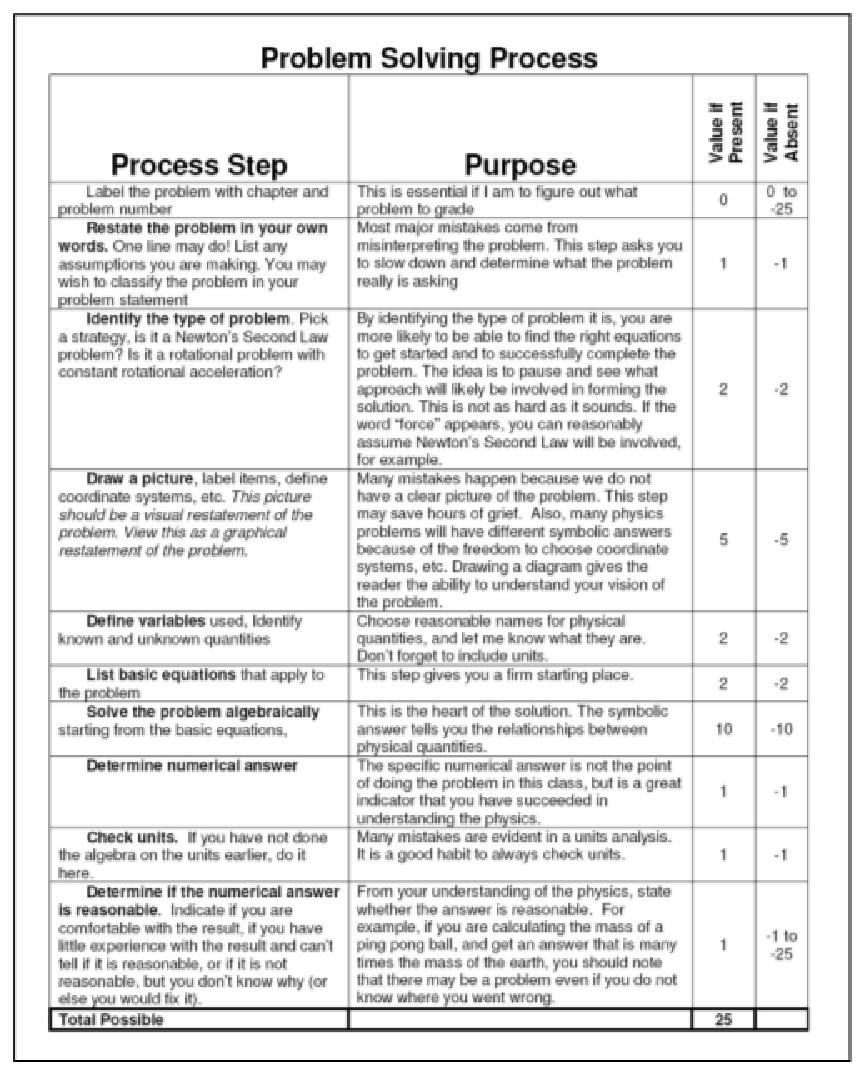
\includegraphics[width=0.5\textwidth]{Problem_Solving_Process}	
		\caption{Problem Solving Process}
		\label{fig:PSP}
	\end{center}
\end{figure}


\section{Restate the Problem}

The first thing to do when working a homework problem (or a problem given to
you in your job, or a problem to test with an experiment, or whatever
problem you are assigned to solve), is to restate the problem. You don't get
as many points if you solve a different problem than was asked! It is
common, especially on tests, to misread the problem. So take some time and
make sure you are answering what was asked. In industry, I used to email my
boss a restatement of each assignment to make sure I\ understood what I had
been assigned!

\section{Identify the type of Problem}

If you can look at the problem and see it as part of a class of problems,
then you know which equations to try, and what techniques to attempt. So far
all we have are displacement, velocity, and acceleration problems. But soon
we will have many other types.

Suppose you are asked to find the displacement of an object that starts at
position $x_{i}=5\unit{m}$ and ends at position $x_{f}=12\unit{m}.$ The
equation 
\begin{equation*}
	\overrightarrow{\mathbf{a}}=\frac{\overrightarrow{\Delta \mathbf{v}}}{\Delta
		t}
\end{equation*}%
is a great resource if you are looking for acceleration, but not so great if
you trying to find the displacement. Identifying that the problem asks for
displacement helps you realize that the equation 
\begin{equation*}
	\Delta x=x_{f}-x_{i}
\end{equation*}%
might help.

\section{Drawing the question}

We have spent three lectures learning how to draw diagrams describing
motion. We will spend more lectures learning how to draw diagrams for force
problems, and equilibrium problems, and rotational problems. You would think
it was an art class!

But seriously, learning to express the problem as a visualization is a large
part of \textquotedblleft doing physics,\textquotedblright\ and the diagram
is often the key to seeing how to solve the problem. It is tempting to skip
this step. But you must convince yourself to learn how to make the diagrams
and to use the diagrams in solving problems.

\subsection{Coordinate Systems}

We need a context in which to describe motion graphically. Like a city map,
there needs to be a way to tell where we are going and where we have come
from. In a western city, we often find a city grid with addresses marked
with a number of streets from a central location. Here in Rexburg we have
such a system. We have addresses like 300N and 200E. We need such a system
for our use.

Often we will use a Cartesian coordinate system (much like the Rexburg
system, which is patterned after a Cartesian system).

We have used this system already in our diagrams (even in the context of
city blocks).

\begin{figure}[h!]
	\begin{center}
		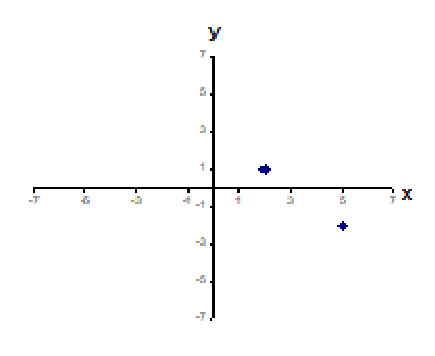
\includegraphics[width=0.3\textwidth]{Coordinate_System_1}	
		\label{fig:Cartesian}
	\end{center}
\end{figure}
We could also make a coordinate system by using the distance from the origin
and an angle from the x-axis. 

\begin{figure}[h!]
	\begin{center}
		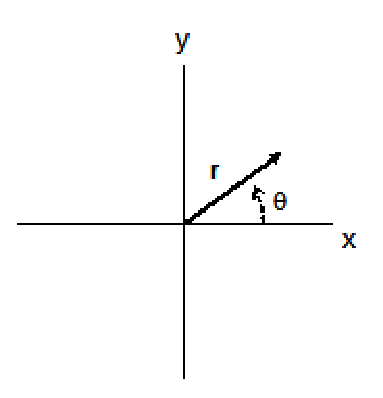
\includegraphics[width=0.3\textwidth]{Coordinate_System_Polar}	
		\label{fig:}Polar
	\end{center}
\end{figure}

I'm sure
you will recognize this as the polar coordinate system. And of course you
recognize our position vectors as just position expressed in polar
coordinates!

We could extend these to three dimensions (and we will later). Einstein used
a very complicated curved three dimensional coordinate system to describe
General Relativity. So what seems like a simple idea can become very
complicated. Fortunately, we can usually use Cartesian coordinates for most
of what we will do.

We will need to think about coordinates a bit. Is there really a zero point
in the universe? If not, then are we always free to choose one?

For distances, we do not believe there is a ultimate zero point. When we get
to other quantities (like temperature) we will see that sometimes there is a
physical zero point.


We have already noticed that our position vector is really just a use of
polar coordinates. And in remembering polar coordinates, you probably recall
that there is trigonometry involved.

Given the triangle below, we recall that 

\begin{figure}[h!]
	\begin{center}
		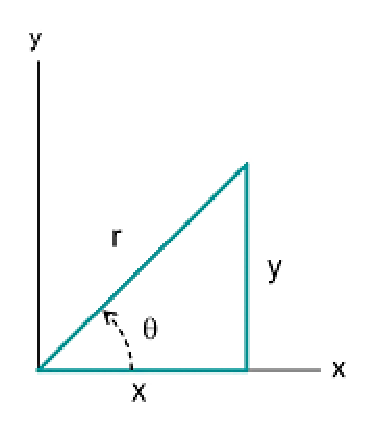
\includegraphics[width=0.3\textwidth]{Triangle}	
		\caption{Triangle}
		\label{fig:Triangle}
	\end{center}
\end{figure}

\begin{equation}
	\sin \left( \theta \right) =\frac{\text{side opposite }\theta }{\text{%
			hypotenuse}}=\frac{y}{r}
\end{equation}

\begin{equation}
	\cos \left( \theta \right) =\frac{\text{side adjacent to }\theta }{\text{%
			hypotenuse}}=\frac{x}{r}
\end{equation}

\begin{equation}
	\tan \left( \theta \right) =\frac{\text{side opposite }\theta }{\text{side
			adjacent to }\theta }=\frac{y}{x}
\end{equation}

Suppose I know $r$ and $\theta $ but not $y,$ I can find $y$ using%
\begin{equation}
	y=r\sin \left( \theta \right)
\end{equation}

We can use cosine and tangent in a similar way.

Suppose we know $r$ and $y,$ but not $\theta .$ We can find this using%
\begin{equation}
	\theta =\arcsin \left( \frac{y}{r}\right)
\end{equation}%
which is often written as%
\begin{equation}
	\theta =\sin ^{-1}\left( \frac{y}{r}\right)
\end{equation}

Also recall the Pythagorean theorem%
\begin{equation}
	r^{2}=x^{2}+y^{2}
\end{equation}

The combination of these ideas will be used over and over in our study of
vectors. If you are a little rusty with trig, it is a good idea to look at
the review in the back of our text book.

A nice way to remember the trig functions is to think of our triangle
inscribed in a unit circle. The cosine of the angle gives the projection of $%
r$ onto the $x$ axis. Likewise, the sine functions the projection of $r$
onto the $y$ axis.

\begin{figure}[h!]
	\begin{center}
		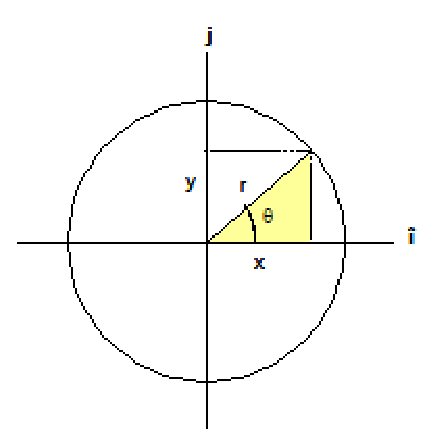
\includegraphics[width=0.3\textwidth]{Unit_Circle}	
		\label{fig:Unit_Circle}
	\end{center}
\end{figure}

As an example of the use of trig functions, we can use them to convert from
Cartesian coordinates $(x,y)$ to polar coordinates $\left( r,\theta \right) $%
. We start with 
\begin{equation}
	r=\sqrt{x^{2}+y^{2}}
\end{equation}%
from the Pythagorean theorem,

Then we note that 
\begin{equation}
	\tan \left( \theta \right) =\frac{x}{y}
\end{equation}%
to yield%
\begin{equation}
	\theta =\tan ^{-1}\left( \frac{x}{y}\right)
\end{equation}

You probably remember that we divide circles into angles as shown in the
figure above. We often divide the circle into $360\unit{%
	%TCIMACRO{\U{b0}}%
	%BeginExpansion
	{{}^\circ}%
	%EndExpansion
},$ like 360 pieces of pizza. By adding up $360^{th}$'s if a circle we can
describe larger angles. This is one way to describe angles. If you took
trigonometry, you remember that there are other ways to divide the circle.
One that will be very important to us is the \emph{radian}. It is just a
slightly bigger pizza piece as a base unit (think of pizza pieces for large
foot ball players, you want to start with larger basic units for them!).
Your calculator will do trigonometry in degrees or radians, but you have to
change the settings to tell the calculator which you want. We will deal with
radians a great deal later, but for now you should find out how to set your
calculator in degrees mode.

\section{Defining Variables}

\begin{figure}[h!]
	\begin{center}
		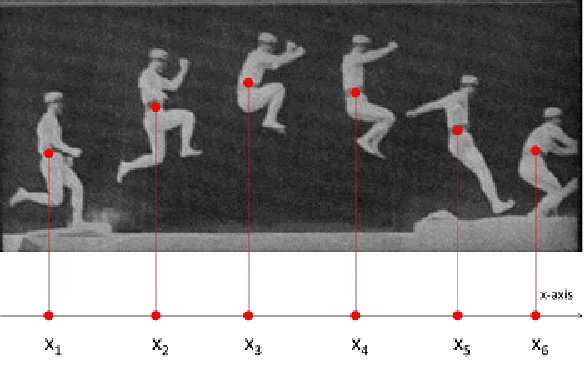
\includegraphics[width=0.8\textwidth]{Jumping_Man}			
		\label{fig:Jumping_Man}
	\end{center}
\end{figure}

Let's look at our jumping man again. It is a great help to realize what you
know. Suppose that we know $x_{i}=5\unit{m}$ and $x_{f}=12\unit{m}$ for our
man. And suppose we want to find the man's total displacement. It is much
easier to see the known values if we call them out 
\begin{eqnarray*}
	x_{i} &=&5\unit{m} \\
	x_{f} &=&12\unit{m}
\end{eqnarray*}

By placing these on your paper so you can see them, it is easier to find an
answer. Seeing the positions like this it is obvious that all you need to do
is subtract to get the answer. As the problems become more complicated, this
will be an even more important step. It also lets the grader (or in your
job, the reader of your report) know what the variable symbols mean. Not
every field uses the same letters for the same quantities. And we reuse some
letters! The letter $T$ could be \textquotedblleft
tension\textquotedblright\ or \textquotedblleft period of
oscillation.\textquotedblright\ By writing down what the letters mean, you
avoid confusing yourself and others.

But what kinds of things are variables? Let's take some time to see what
quantities we might define.

\subsection{Objects}

We have been talking about objects, like our jumping man, the bird, or a
ball. But what is an object? What is the universe made of?

The startling answer is, we're not entirely sure! Oh, we know that the
universe is made of stars and planets and galaxies and dust and many other
things, but what are the things made of?

Answering that question is the job of particle physics, and the answer is
still in the making. For our study of motion, we will assume there are
fundamental things in the universe, and more complicated things are made of
these fundamental things. Lets look at three quantities as our initial
building blocks. \emph{Mass, Length}, and \emph{Time}.

\subsubsection{Mass}

When we think of an object, we usually think of something that has mass.
Mass is an amount of matter. Exactly what matter is, still somewhat of a
question (Job security for Physicists). Einstein equated mass and energy.
The great experiments at the Conseil Europ\'{e}en pour la Recherche Nucl\'{e}%
aire (CERN) are trying to understand exactly what mass is. You may have
heard of the \emph{Higgs boson}, a particle discovered at CERN that gives us
a hint that our theory of what mass is might be right. But that is current
on-going research. So for this class we shall take mass as just the amount
of matter and trust our intuition on what that means. The standard unit of
mass is the kilogram, abbreviated \textquotedblleft $\unit{kg}.$%
\textquotedblright\ It is the mass of a standard piece of platinum alloy,
again kept in France. 

\begin{figure}[h]
	\begin{center}
		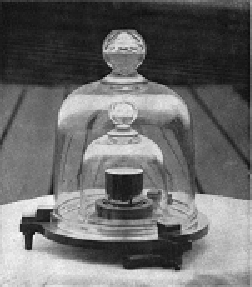
\includegraphics[width=0.3\textwidth]{Kilogram}			
		\caption{US National Institute of Standards standard kilogram.}
		\label{fig:kilogram}
	\end{center}
\end{figure}

Note that mass and weight are very different quantities. you can see this if
we use a bathroom scale. On earth the scale gives a reading that is
proportional to the amount of matter in our bodies, but if we put it on a
space craft in orbit, it would not measure any weight at all. Yet the amount
of matter in our bodies has not changed!%


\subsubsection{Length}

Perhaps we should really say \textquotedblleft space\textquotedblright\
here. We need to have some idea of how far away things are or how long or
tall things are. In this class our view of space will be that it is a
container in which things happen. When you study Einstein's Relativity we
will change that a little, but for now space is a container, and length is a
measure of how far away in this container something is.

In ancient Egypt, the standard of measuring length was when Pharaoh took his
ceremonial reed and measured the length of the foundation for the temple (a
little like our standard kilogram for mass). This might sound strange, but
in essence this is what we all did until 1960. Prior to this, a meter, our
unit of length, was defined as one ten millionth of the distance from the
North Pole to the equator. Since this was not a very practical day-to-day
measuring device, a standard \textquotedblleft reed\textquotedblright\ (this
time made of platinum) was kept in France, and meter sticks were made to
match this standard. There are terrible problems with this! Each stick of a
different materials changes length with temperature! So in 1983 the meter
was defined as the distance light traves in vacuum during a time interval of 
\begin{equation*}
	\frac{1}{299792458}\unit{s}
\end{equation*}%
The abbreviation for meter is \textquotedblleft $\unit{m}.$\textquotedblright

\subsubsection{Time}

You might object that time is not a thing. But we have already used time in
our study of motion. It must be something! We should define it before we get
to familiar with using time. But what is time? It turns out that time is
hard to define. We usually use the idea that time is how long we wait.%
\footnote{%
	Feynman, Richard, Robert Leighton, Matthew Sands, \emph{The Feynman Lectures
		on Physics}, Vol. I, Addison-Sesley, Reading Massachusetts, 1963} That can
be tricky to measure. Let's start with something simple. How much time will
you spend in this class today? That is a time we can wait, about an hour.
But it is harder to answer questions like \textquotedblleft how long does it
take for light to travel a foot.\textquotedblright\ The answer is about a
nanosecond. We cannot perceive of times this small. Likewise, we cannot wait
for a million years (well, we could, but our vantage point might change
after the first 70 years or so).

To measure time we use events that are \emph{periodic}, that is, they occur
at regular intervals. An early example is the pendulum of a clock. From a
fundamental periodic phenomena, we can build up larger or smaller units of
time.

The current unit is the \emph{second}, abbreviated \textquotedblleft $\unit{s%
},$\textquotedblright\ which is given as $91926317000$ times the period of
oscillation of radiation from the cesium atom. Fortunately we can just use a
clock or watch to measure seconds.

The standard for time is the atomic clock.



	\begin{figure}[h]
		\centering
		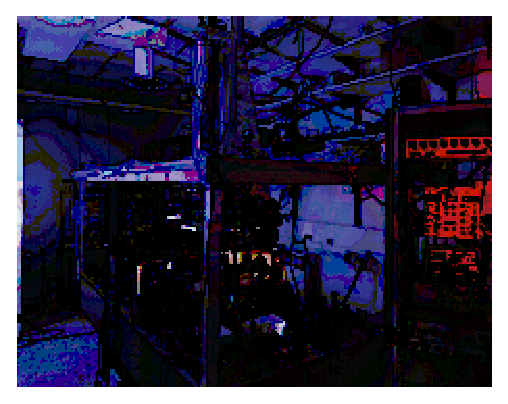
\includegraphics[width=0.5\textwidth]{Atomic_Clock}
		\caption{Atomic Clock}
		\label{fig:AtomicClock}
	\end{figure}



\subsection{Derived quantities}

So we have objects made of mass and space (length) and time to use in
describing their motion.

%TCIMACRO{%
	%\TeXButton{Question 1.1.1}{\marginpar {
			%\hspace{-0.5in}
			%\begin{minipage}[t]{1in}
			%{\color {blue} \small{Question 1.1.1}}
			%\end{minipage}
			%}}}%
%BeginExpansion
\marginpar {
	\hspace{-0.5in}
	\begin{minipage}[t]{1in}
		{\color {blue} \small{Question 1.1.1}}
	\end{minipage}
}%
%EndExpansion
When we combine quantities we derive new quantities that are useful from the
basic length, time, mass set. For example, speed is a combination of length
and time.%
\begin{equation}
	v=\frac{\Delta x}{\Delta t}
\end{equation}%
quantities like acceleration, force, momentum, etc. are derived quantities.

\subsection{Dimensional Analysis}

Analysis of the units in a measurement can be very useful. For example, if
we take our first equation%
\begin{equation}
	v=\frac{\Delta x}{\Delta t}
\end{equation}%
and look at the units, we find that $x$ is a length in, say, meters. We find
that $t$ is a time in, say, seconds. Then when we calculate $v$ we should
have units of $\unit{m}/\unit{s}.$ If, instead, we have $\unit{m}^{3}$ at
the end of our calculation, something must have gone wrong! Sometimes it is
useful to use generic units for our analysis. That is, any length is given a
unit $L$ and any time is given a unit $T.$ So our equation gives 
\begin{equation*}
	\frac{\Delta x}{\Delta t}\Rightarrow \frac{L}{T}
\end{equation*}%
To see this lets take and acceleration . It is given by 
\begin{equation*}
	a=\frac{\Delta v}{\Delta t}\Rightarrow \frac{\frac{L}{T}}{T}=\frac{L}{T^{2}}
\end{equation*}%
so from dimensional analysis, we expect that acceleration would be something
like 
\begin{equation*}
	a=c\frac{x}{t^{2}}
\end{equation*}%
and we could deduce that 
\begin{equation*}
	x=\frac{1}{c}at^{2}
\end{equation*}%
note that I included a constant, $c.$ Dimensional analysis cannot tell you
the constants in an equation. We will see later that in this case $c=2$ so 
\begin{equation*}
	x=\frac{1}{2}at^{2}
\end{equation*}

We will find out that our dimensional analysis did not hit too far off the
mark. This is part of the equation for position for an accelerating object.

\subsection{Units}

No value in physics is useful without a unit. For example, if I tell you to
jump from a height of $100,$ it makes a difference whether it is $100\unit{cm%
}$ or $100\unit{m}!$ Units tell us what standard was used to make the
measurement so all who see the result can correctly interpret what it means.

\subsection{System of Units}

You will notice that we have only given metric units. We will use the \emph{%
	Syst\`{e}me International} or $\emph{SI}$ units. There are, of course, other
systems of units. We will try to ignore them in this class. Occasionally we
may use feet for length and slugs (yes, slugs) for mass. we will usually use
the following SI units for our basic quantities.%
\begin{equation*}
	\begin{tabular}{lll}
		Quantity & Unit & Symbol \\ 
		Mass & Kilogram & $\unit{kg}$ \\ 
		Length & meter & $\unit{m}$ \\ 
		Time & second & $\unit{s}$%
	\end{tabular}%
\end{equation*}

The SI system makes use of prefixes to modify the basic unit, like \emph{%
	centi}meter to mean $1/100$ of a meter. You should be familiar with the
following prefixes.\medskip 
\begin{equation*}
	\begin{tabular}{|l|l|l|l|l|l|l|}
		\hline
		Prefix & Symbol & Power &  & Prefix & Symbol & Power \\ \hline
		nano- & n & $10^{-9}$ &  & giga- & G & $10^{9}$ \\ \hline
		micro- & $\mu $ & $10^{-6}$ &  & mega- & m & $10^{6}$ \\ \hline
		mili- & m & $10^{-3}$ &  & kilo- & k & $10^{3}$ \\ \hline
		centi- & c & $10^{-2}$ &  & deka- & da & $10^{1}$ \\ \hline
		deci- & d & $10^{-1}$ &  &  &  &  \\ \hline
	\end{tabular}%
\end{equation*}

We can already see that our unit for mass, the kilogram, must be 1000 grams.
A centimeter must be $1/100^{th}$ of a meter. We obviously will need to be
able to convert from centimeters to meters from time to time. We should be
able to convert from any prefixed unit to any other prefixed unit. We nee a
strategy to do this.

\subsection{Unit Conversions}

Let's do a unit conversion that most of you do in your head. Let's convert
hours to seconds. We know that 
\begin{equation*}
	1\unit{h}=60\unit{min}
\end{equation*}%
and we know that 
\begin{equation*}
	1\unit{min}=60\unit{s}
\end{equation*}%
Suppose we have $5$ hours. How many seconds is this?

Most of us would say multiply by $3600,$ and that is right, but let's do it
one step at a time so you can see the process. I\ want to multiply $5$ by
something, but I\ can't change the duration. At the end of our calculation,
it still has to be a wait of $5\unit{h}$ even though we now give the value
in seconds. For a person waiting $5$ hours and a second one waiting $%
\allowbreak 18\,000\unit{s}$ they must feel the same amount of time. So we
need to adjust our $5$ hours by something that does not change the wait.

I\ think you will agree that if I\ multiply by $1$ nothing changes%
\begin{equation*}
	5\times 1=5
\end{equation*}%
We can do this with units%
\begin{equation*}
	5\unit{h}\times 1=5\unit{h}
\end{equation*}%
now let's take our equation relating hours to minutes.%
\begin{equation*}
	1\unit{h}=60\unit{min}
\end{equation*}%
and let me divide by $1\unit{h}$%
\begin{eqnarray*}
	\frac{1\unit{h}}{1\unit{h}} &=&\frac{60\unit{min}}{1\unit{h}} \\
	1 &=&\frac{60\unit{min}}{1\unit{h}}
\end{eqnarray*}%
I can multiply by the right hand side of this equation and all I am doing is
multiplying by $1!$%
\begin{equation*}
	5\unit{h}\times \frac{60\unit{min}}{1\unit{h}}=5\unit{h}
\end{equation*}%
This still must be true, but let's do the math%
\begin{equation*}
	5\unit{h}\times \frac{60\unit{min}}{1\unit{h}}=\allowbreak 300\unit{min}
\end{equation*}%
this is how many minutes are in $5$ hours. We can play the same trick with
minutes to seconds%
\begin{eqnarray*}
	\frac{1\unit{min}}{1\unit{min}} &=&\frac{60}{1\unit{min}}\unit{s} \\
	1 &=&\frac{60\unit{s}}{1\unit{min}}
\end{eqnarray*}%
so we can take our $300\unit{min}$ and find out how many seconds we have!%
\begin{equation*}
	\allowbreak 300\unit{min}\times \frac{60\unit{s}}{1\unit{min}}=18000.0\unit{s%
	}
\end{equation*}%
Now we could do this all in one equation, using our strange way of writing $%
1 $ that converts from hours to minutes and our strange way of writing $1$
that converts from minutes to seconds. 
\begin{eqnarray*}
	5\unit{h}\times 1\times 1 &=&5\unit{h} \\
	5\unit{h}\times \frac{60\unit{min}}{1\unit{h}}\frac{60\unit{s}}{1\unit{min}}
	&=&18000.0\unit{s}
\end{eqnarray*}%
Notice that the units cancel like variables in algebra!

We will treat units like algebraic quantities that can be canceled. Let's do
another example. We want to convert $10\unit{mi}$ (ten miles) to kilometers.
We know that 
\begin{equation}
	1\unit{mi}=1609\unit{m}
\end{equation}%
and we know that 
\begin{equation}
	1\unit{km}=1000\unit{m}
\end{equation}%
Start with conversion from miles to meters. We recognize that with a small
use of algebra 
\begin{equation}
	1=\frac{1609\unit{m}}{1\unit{mi}}
\end{equation}%
then we can write 
\begin{equation}
	10\unit{mi}=10\unit{mi}\frac{1609\unit{m}}{1\unit{mi}}=\allowbreak 16\,090%
	\unit{m}
\end{equation}

Then we also recognize that 
\begin{equation}
	1=\frac{1000\unit{m}}{1\unit{km}}
\end{equation}%
or%
\begin{equation}
	1=\frac{1\unit{km}}{1000\unit{m}}
\end{equation}%
then%
\begin{equation}
	\allowbreak 16\,090\unit{m}=16\,090\unit{m}\frac{1\unit{km}}{1000\unit{m}}%
	=\allowbreak 16090.0\unit{m}
\end{equation}

so 
\begin{equation}
	10\unit{mi}=16\unit{km}
\end{equation}

We could do this all in one large, chained, conversion%
\begin{equation}
	10\unit{mi}=10\unit{mi}\frac{1609\unit{m}}{1\unit{mi}}\frac{1\unit{km}}{1000%
		\unit{m}}=16\unit{km}
\end{equation}

If you think about it, to convert units, we have multiplied by $1$ several
times. So as you multiply to convert units, make sure your factors multiply
are equal to $1.$

\subsection{Uncertainty in measurements}

In science, we must face the fact that no measurement is completely
accurate. The reasons for uncertainty are limitations in our human sensory
system or sensing apparatus. For example, if I measure a square of metal
with a ruler. I am likely not able to tell the length to better than a tenth
of a centimeter ($1\unit{mm}$). This is because of inaccuracies in the ruler
and in my own ability to see the ruler clearly and consistently. So suppose
I\ have a measurement of $16.3\unit{cm}$. I can really only tell you that
the measurement is between $16.4\unit{cm}$ and $16.2\unit{cm}.$ we could
write this as $16.3\pm 0.1\unit{cm}.$ We will study uncertainty in
measurements in some detail in PH150. But for PH121 we will need some
provisional rules that let us make a guess on now good our answers are.

\subsubsection{Significant figures}

Scientists have devised a clever way to include the level of uncertainty in
the statement of the measurement result. This is referred to as \emph{%
	significant figures} and it basically means to keep only the digits in a
number that contain well known information. In the above example, we would
say that in $16.3\unit{cm}$ that the $3$ is the least significant digit. Now
suppose we use the same ruler to measure the same object, but I\ tell you
that the measurement is $16.3259357\unit{cm}.$ If we know the measurement is
only good to $\pm 0.1\unit{cm},$ what can we say about the digits $259357?$
We can say they are worthless! They are nonsense, so we cleverly leave them
off! There are a series of rules to tell us which digits are significant. It
is important to realize that zeros that just mark where the decimal place
goes are not significant (e.g. in $0.00163\unit{cm}$ the three $0$'s are not
significant, but in $1.400\unit{cm}$ the digits mean that the measurement is
known to $\pm 0.001\unit{cm}$).

We usually express numbers in scientific notation.

\subsubsection{Propagation of uncertainty}

Suppose we take two measurements, like measuring the sides of a rectangle. 
\begin{eqnarray*}
	l &=&\left( 2.3\pm 0.1\right) \unit{cm} \\
	w &=&\left( 4.5\pm 0.1\right) \unit{cm}
\end{eqnarray*}%
and we wish to find the area%
\begin{equation*}
	A=l\times w
\end{equation*}%
\begin{eqnarray*}
	A &=&2.3\unit{cm}\times 4.5\unit{cm} \\
	&=&\allowbreak 10.\,\allowbreak 35\unit{cm}^{2}
\end{eqnarray*}%
But we were a little uncertain about the length and width, wouldn't we also
be uncertain about the area that we made from the uncertain length and the
width? Of course there is some uncertainty in the area. Let's see how we
could deal with this.

The length could have been as much as 
\begin{equation*}
	l=2.3\unit{cm}+0.1\unit{cm}=2.\,\allowbreak 4\unit{cm}
\end{equation*}%
and the width could be as much as 
\begin{equation*}
	w=\left( 4.5+0.1\right) \unit{cm}=4.\,\allowbreak 6\unit{cm}
\end{equation*}%
So the area could be as much as 
\begin{eqnarray*}
	A_{+} &=&2.4\unit{cm}\times 4.6\unit{cm} \\
	&=&\allowbreak 11.\,\allowbreak 04\unit{cm}^{2}
\end{eqnarray*}%
But the length could be as little as 
\begin{equation*}
	l=2.3\unit{cm}-0.1\unit{cm}=2.2\unit{cm}
\end{equation*}%
and the width could be as little as 
\begin{equation*}
	w=\left( 4.5-0.1\right) \unit{cm}=4.4\unit{cm}
\end{equation*}%
So the area could be as little as%
\begin{eqnarray*}
	A_{-} &=&2.2\unit{cm}\times 4.4\unit{cm} \\
	&=&\allowbreak 9.\,\allowbreak 68\unit{cm}^{2}
\end{eqnarray*}

We can see that these differ by about $\pm 1\unit{cm}^{2}$ total. 
\begin{equation*}
	A_{+}-A_{-}=11.\,\allowbreak 04\unit{cm}^{2}-\allowbreak \allowbreak
	9.\,\allowbreak 68\unit{cm}^{2}=1.\,\allowbreak 36\unit{cm}^{2}
\end{equation*}%
Thus the tenths and hundredths places in our calculated area cannot be very
certain. We drop these and write%
\begin{equation*}
	A=\allowbreak 10\pm 1\unit{cm}
\end{equation*}%
Notice that our length and width had two digits, 
\begin{eqnarray*}
	l &=&\left( 2.3\pm 0.1\right) \unit{cm} \\
	w &=&\left( 4.5\pm 0.1\right) \unit{cm}
\end{eqnarray*}%
with the uncertainty in the second digit, and notice that our answer for the
area has two digits, and the uncertainty is in the second digit!

In general:

\begin{quotation}
	\emph{In multiplying or dividing two quantities, the number of significant
		figures in the product or quotient is the same as the number of significant
		figures in the least accurate of the factors being combined. }
\end{quotation}

In our example, $l$ and $w$ both have two significant figures, so the result
should be limited to two significant figures

For addition and subtraction the rules is:

\begin{quotation}
	\emph{The number of decimal places in the result should equal the smallest
		number of decimal places in any term in the sum or difference}.
	
	These two rules will help us determine how many digits to keep for most
	problems. You may know that there are several other rules, and thought we
	wont derive them like we did for multiplication, we will use them in our
	problems. Here they are in a table%
	\begin{equation*}
		\begin{tabular}{|l|}
			\hline
			{\small \qquad \qquad \qquad \qquad \qquad \qquad \qquad \qquad }\textbf{%
				Significant Figure Rules} \\ \hline
			{\small \quad 1. Non-zero digits are always significant} \\ \hline
			{\small \quad 2. Embedded (i.e. captive) zero-digits are always significant}
			\\ \hline
			{\small \quad 3. For the }$number${\small \ zero only the zero-digits after
				the decimal are significant} \\ \hline
			{\small \quad 4. Leading zero-digits are not significant} \\ \hline
			{\small \quad 5. Trailing zero digits:} \\ \hline
			{\small \qquad If the number has a decimal, the trailing zero digits are
				significant} \\ \hline
			{\small \qquad If the number does not have a decimal, the trailing zero
				digits are not significant} \\ \hline
			\begin{tabular}{l}
				{\small 6. The final result of multiplication or division operation should
					have the same number } \\ 
				{\small \quad of significant digits as the measured quantity with the least
					number of significant } \\ 
				{\small \quad figures used in the calculation.}%
			\end{tabular}%
			{\small \ } \\ \hline
			\begin{tabular}{l}
				{\small 7. The final result of an addition or subtraction operation should
					have the same number } \\ 
				{\small \quad\ digits to the right of the decimal as the measured quantity
					with the least number of } \\ 
				{\small \quad\ decimal used in the calculation. }%
			\end{tabular}%
			{\small \ } \\ \hline
			{\small 
				\begin{tabular}{l}
					8. For a mixture of operations, work from left to right, do mathematical
					hierarchy of operations \\ 
					\quad\ ($\times $\ or $\div ,$\ then $+$\ or $-$).%
				\end{tabular}
			} \\ \hline
		\end{tabular}%
	\end{equation*}
\end{quotation}

\section{Basic Equations}

Equations are relationships in physics. The equation 
\begin{equation*}
	\overrightarrow{\mathbf{v}}=\frac{\overrightarrow{\Delta \mathbf{x}}}{\Delta
		t}
\end{equation*}%
tells us how the displacement and duration combine to form velocity. These
equations are our way of expressing motion. They are the tools in our
toolbox for solving problems. Once you have identified the type of problem
you have, you can quickly write down a list of equations (tools) that you
could use to solve that problem. You might write down more equations than
you end up using for a particular problem. That's OK. You don't empty your
tool box of all tools but the ones you think you might use when you start a
fix-up job in your house! You should not do so when starting a problem. List
your equations, then choose the ones that seem to work given your known
values in your list of variables.

\section{Solving with symbols}

For years now, you have worked with numbers and answers that are numbers.
And that is what the teacher was looking for. But in physics the equation is
the important thing. It tells you how things relate to each other. Let's try
an example:

\texttt{The initial speed of an object is }$3\unit{m}/\unit{s}$\texttt{\ and
	it's acceleration is }$2\unit{m}/\unit{s}^{2}$\texttt{\ in the same
	direction as the velocity. Find the speed half a second after the experiment
	start.}

We want to start by restating the problem:

\texttt{Find the final speed knowing }$a$\texttt{\ and }$v_{i}$

Next identify the type of problem. I think it is an acceleration problem:

\texttt{PT acceleration}

Next we want to draw the picture

\begin{figure}[h!]
	\begin{center}
		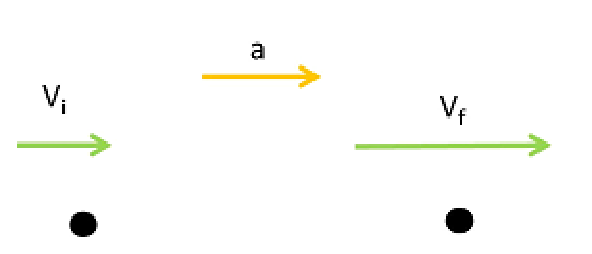
\includegraphics[width=0.7\textwidth]{Moving_Object_Velocity_Acceleration}			

		\label{fig:Moving_Object_Velocity_Acceleration}
	\end{center}
\end{figure}

Our variables list is next:

\texttt{VAR}

\begin{eqnarray*}
	v_{i} &=&3\frac{\unit{m}}{\unit{s}} \\
	a &=&2\frac{\unit{m}}{\unit{s}^{2}} \\
	\Delta t &=&0.5\unit{s}
\end{eqnarray*}

and now basic equations:

\texttt{BE:}

\begin{equation*}
	\underline{\overrightarrow{\mathbf{a}}}=\frac{\overrightarrow{\Delta \mathbf{%
				v}}}{\underline{\Delta t}}
\end{equation*}%
\begin{equation*}
	\overrightarrow{\Delta \mathbf{v}}=\overrightarrow{\mathbf{v}}_{f}-%
	\underline{\overrightarrow{\mathbf{v}}_{i}}
\end{equation*}%
\begin{equation*}
	\overrightarrow{\mathbf{v}}=\frac{\overrightarrow{\Delta \mathbf{x}}}{\Delta
		t}
\end{equation*}%
\begin{equation*}
	\overrightarrow{\Delta \mathbf{x}}=\overrightarrow{\mathbf{x}}_{f}-%
	\overrightarrow{\mathbf{x}}_{i}
\end{equation*}%
Note that I\ underlined the known values from my list variables. The first
two equations have $v_{f}$ in them and they contain my known values, so it
looks like they are the ones to use in my solution.

\subsection{Solve Algebraically}

Now we try to solve for the speed, but we do so symbolically. We already
believe that the first two equations in our basic equation list will be
helpful, so let's start with 
\begin{equation*}
	\underline{\overrightarrow{\mathbf{a}}}=\frac{\overrightarrow{\Delta \mathbf{%
				v}}}{\underline{\Delta t}}
\end{equation*}%
and put in 
\begin{equation*}
	\overrightarrow{\Delta \mathbf{v}}=\overrightarrow{\mathbf{v}}_{f}-%
	\underline{\overrightarrow{\mathbf{v}}_{i}}
\end{equation*}

\begin{equation*}
	\underline{\overrightarrow{\mathbf{a}}}=\frac{\overrightarrow{\mathbf{v}}%
		_{f}-\underline{\overrightarrow{\mathbf{v}}_{i}}}{\underline{\Delta t}}
\end{equation*}%
At this point I\ recognize that I\ can solve for $v_{f}$ and everything else
is known. I could plug things in my calculator and have it solve for $v_{f}$
using numbers, but we won't do that! We will continue with algebra 
\begin{equation*}
	\overrightarrow{\mathbf{a}}\Delta t=\overrightarrow{\mathbf{v}}_{f}-%
	\overrightarrow{\mathbf{v}}_{i}
\end{equation*}%
and%
\begin{equation*}
	\overrightarrow{\mathbf{a}}\Delta t+\overrightarrow{\mathbf{v}}_{i}=%
	\overrightarrow{\mathbf{v}}_{f}
\end{equation*}%
or%
\begin{equation*}
	\overrightarrow{\mathbf{v}}_{f}=\overrightarrow{\mathbf{v}}_{i}+%
	\overrightarrow{\mathbf{a}}\Delta t
\end{equation*}%
Since $\overrightarrow{\mathbf{a}}$ and $\overrightarrow{\mathbf{v}}_{i}$
are in the same direction, their magnitudes just add so 
\begin{equation*}
	v_{f}=v_{i}+a\Delta t
\end{equation*}

\textbf{This is the symbolic answer.} It has the thing I\ want, $v_{f},$ an
equals sign, and then symbols for what $v_{f}$ is equal to.

\section{Numeric answer}

The numeric answer is easy. Just plug in numbers to your symbolic answer%
\begin{equation*}
	v_{f}=v_{i}+a\Delta t
\end{equation*}%
\begin{eqnarray*}
	v_{f} &=&3\frac{\unit{m}}{\unit{s}}+\left( 2\frac{\unit{m}}{\unit{s}^{2}}%
	\right) \left( 0.5\unit{s}\right) \\
	&=&4.0\frac{\unit{m}}{\unit{s}}
\end{eqnarray*}

\section{Reasonableness check}

If we had gotten $400000000000\unit{m}/\unit{s}$ in our example, we would
know something went wrong. Nothing can go this fast! It is good to check
your answer and see if it seems to make sense. But how do we do that? One
way is to do a quick estimate.

\subsection{Estimates}



There are times when we simply do not have all the information we need, but
we need a number for something anyway. There are also times when we wish to
make a quick calculation (like checking on the reasonableness of a
calculation). In such cases, we estimate. Many people in science are
somewhat uncomfortable with estimates, because they are not
\textquotedblleft correct\textquotedblright\ (In business and politics,
people may be a little too comfortable with estimates).

Let's do a few examples together.

\subsubsection{Example 1: How many sheets of paper fit between the Earth and
	Moon?}

To do this calculation, we need to know how far away the Moon is and how
thick a piece of paper is.%
\begin{equation}
	D_{EM}=4000000\unit{km}
\end{equation}%
\begin{eqnarray}
	t &=&\frac{3\unit{mm}}{28}=1.\,\allowbreak 071\,4\times 10^{-4}\unit{m} \\
	&\approx &\allowbreak 1\times 10^{-4}\unit{m}  \notag
\end{eqnarray}

so the number of pieces of paper would be%
\begin{eqnarray}
	N &=&\frac{D_{EM}}{t}=\frac{4000000\unit{km}}{1\times 10^{-4}\unit{m}}\frac{%
		1000\unit{m}}{\unit{km}} \\
	&=&40\,000\,\allowbreak 000\,000\,000  \notag \\
	&=&4.0\times 10^{13}  \notag \\
	&\approx &1\times 10^{13}
\end{eqnarray}

Is this reasonable? Well look at Example 1.7 in the book and see what you
think (and explain why our answers are different).

\subsubsection{Example 2 How much sand is in the world's beaches?}

\begin{figure}[h!]
	\begin{center}
		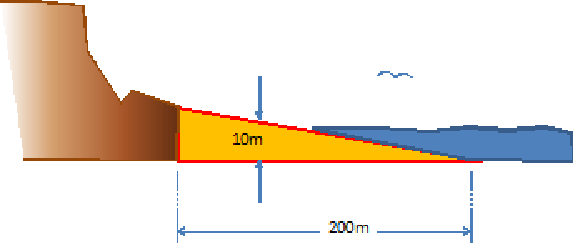
\includegraphics[width=0.7\textwidth]{Beach}			
		\label{fig:Beach}
	\end{center}
\end{figure}





We start by looking for a fundamental element of a beach, say, a grain of
sand. We can calculate the total volume of the beaches, and divide by the
volume of a grain of sand. This will tell us how many grains of sand there
are in the world's beaches. If we can get an estimate of the mass of a grain
of sand, then we can answer how much sand is in the world's beaches.

Lets estimate the grain of sand to have a mass of 
\begin{equation}
	m=0.005\unit{kg}
\end{equation}%
Let's guess a volume of%
\begin{equation}
	V_{s}=\allowbreak 1.0\times 10^{-15}\unit{m}^{3}
\end{equation}
We can estimate the length of the world's coastline to be%
\begin{equation}
	L=40000000000\unit{m}
\end{equation}%
we need the volume of the coast line, lets say the beach is 
\begin{equation}
	w=200\unit{m}
\end{equation}
wide and 
\begin{equation}
	d=10\unit{m}
\end{equation}
deep.

Then the volume of the world's beaches would be%
\begin{eqnarray}
	V &=&Lwd=\left( 40000000000\unit{m}\right) \left( 200\unit{m}\right) \left(
	10\unit{m}\right) \\
	&=&8.0\times 10^{13}\unit{m}^{3}
\end{eqnarray}
and the number of grains of sand would be%
\begin{equation}
	N=\frac{V}{V_{s}}=\frac{Lwd}{V_{s}}=\allowbreak 8.0\times 10^{28}
\end{equation}

which gives us%
\begin{eqnarray}
	M_{beach} &=&Nm=\left( \allowbreak 8.0\times 10^{28}\right) \left( 0.005%
	\unit{kg}\right) \\
	&=&4.0\times 10^{26}\unit{kg}
\end{eqnarray}

Mass of the Earth

\begin{equation}
	M_{E}=5.98\times 10^{24}\unit{kg}
\end{equation}

where did we go wrong?

Consider silicon oxide. It has a density of 
\begin{equation}
	\rho =2200\frac{\unit{kg}}{\unit{m}^{3}}
\end{equation}%
If our estimate of 
\begin{equation}
	m=0.005\unit{kg}
\end{equation}%
is good, then we should have used a volume of%
\begin{eqnarray}
	V &=&\frac{m}{\rho }=\frac{0.005\unit{kg}}{2200\frac{\unit{kg}}{\unit{m}^{3}}%
	} \\
	&=&2.\,\allowbreak 272\,7\times 10^{-6}\allowbreak \unit{m}^{3}
\end{eqnarray}%
So one problem is that our estimate of the volume of a grain of sand is very
bad.

In general, you can be creative in making estimates, but you do have to be
careful.

\section{Units Check}

We already have discussed units. But it is important to check your units in
your final answer. In our case, the final units must be a length unit
divided by a time unit. For speed this must be the case. If we had gotten a
length unit divided by a time squared, then we would know something went
wrong in our algebra. If the units don't work the answer is wrong. So
especially on a test (or in your real job) checking units is important!

\section{Problem Solving Process}

I have assembled all of the problem solving pieces that we have studied into
a process that leads us to our solution. Here is the process we will use in
a table:

\begin{figure}[h!]
	\begin{center}
		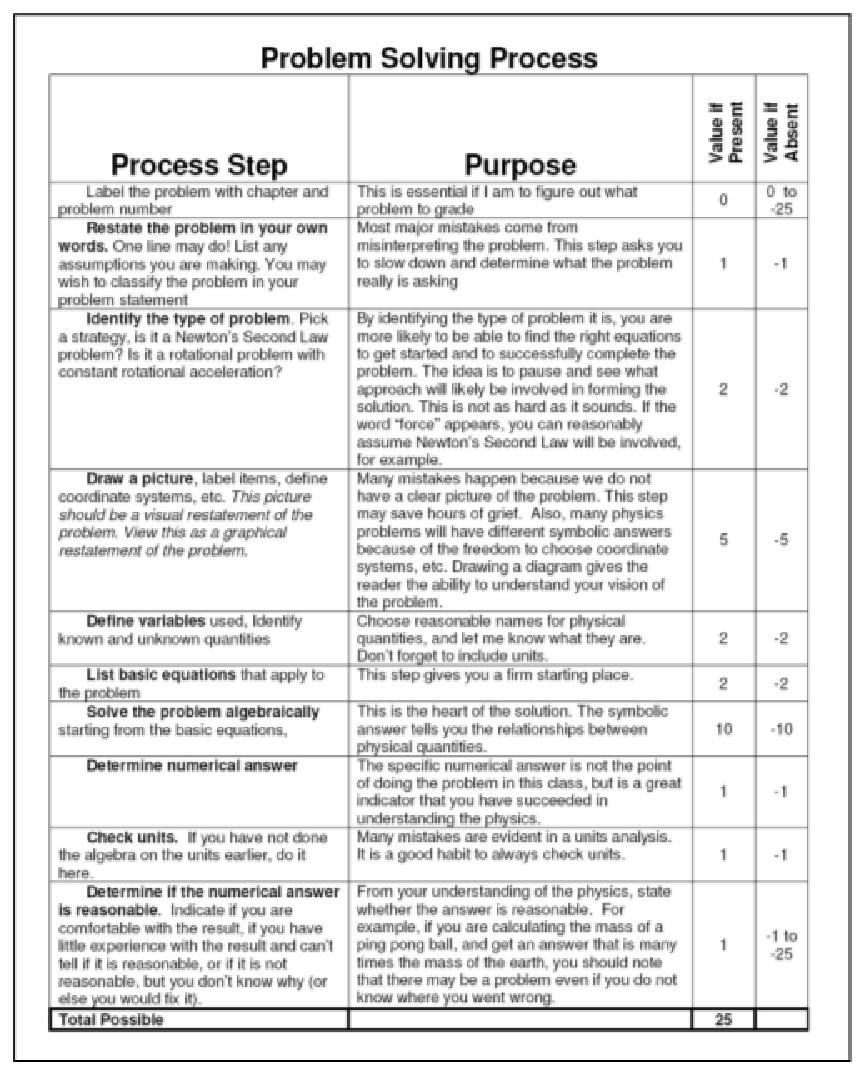
\includegraphics[width=0.8\textwidth]{Problem_Solving_Process}	
		\label{fig:PSP2}
	\end{center}
\end{figure}

Notice that I have assigned point values to each part. So if you leave out a
part you will know how many points you will miss. Also notice that there are
a lot of points for the symbolic answer and only a one for the numeric
answer. Physics is about relationships that describe motion, the numbers
just aren't that important. So it is not a winning strategy to only give me
the numeric answer for a problem. you only get one out of twenty five points!

Also notice that if I\ ask for the mass of a ping pong ball, and you give me
an answer that is three times the mass of Jupiter, I\ can take off more than
one point for the very wrong numeric answer! Since you will be doing a
reasonableness check, you won't have this problem. But what if you don't
know if an answer is reasonable? Then say you don't know! You will act
differently as a physicist, engineer, doctor, etc. if you admit in your
calculations that you are not certain of the result. And this is very
valuable! It can save your job! So if you are not sure, say so.

We will use this process for the rest of the semester, and this or a similar
process for PH123, and PH220 (or PH223) and if you are a physicist for the
rest of your career. This is also the process I used in engineering in
industry. So it is worth practicing in our problems. It is also how I\ will
grade the tests!
 

 \appendix


 \bibliographystyle{phBYU}
 \bibliography{orbits}

 
% \phantomsection \addcontentsline{toc}{chapter}{Index}
  \renewcommand{\baselinestretch}{1} \small \normalsize
  \printindex


\end{document}
